% TODO:
% Discussion of interaction between inbound protocol governor and connection
% manager when a new outbound connection is requested.

% TODO:
% I realised that it would be nicer to structure the spec a bit differently.
% First describe each transition in general terms, without referring to the
% implementation, and in a subsequent section introduce implementation details.

\chapter{Connection Manager State Machine Specification}
\label{chapter:connection-manager}

\tikzstyle{decision} =
  [ diamond
  , fill=DarkSeaGreen1
  , text width=4.5em
  , text badly centered
  , node distance=3cm
  , inner sep=0pt
  ]
\tikzstyle{outbound_state} =
  [ rectangle
  , rounded corners
  , fill=DodgerBlue1
  , minimum height=2em
  ]
\tikzstyle{inbound_outbound_state} =
  [ rectangle
  , rounded corners
  , fill=HotPink3
  , minimum height=2em
  ]
\tikzstyle{inbound_state} =
  [ rectangle
  , rounded corners
  , fill=DarkOliveGreen3
  , minimum height=2em
  ]
\tikzstyle{impossible_outbound_state} =
  [ rectangle
  , rounded corners
  , fill=LightBlue2
  , rounded corners
  , minimum height=2em
  ]
\tikzstyle{line} =
  [ draw
  , -latex'
  ]
\tikzstyle{error} =
  [ rectangle
  , rounded corners
  , fill=red!255!blue!20
  , minimum height=2em
  ]
\tikzstyle{requestOutboundArr}      = [ color = DodgerBlue1 ]
\tikzstyle{registerInboundArr}      = [ color = HotPink3 ]
\tikzstyle{promotedToWarmRemoteArr} = [ color = DarkOliveGreen3 ]
\tikzstyle{demotedToColdRemoteArr}  = [ color = Orange2 ]
\tikzstyle{unregisterOutboundArr}   = [ color = Turquoise ]
\tikzstyle{unregisterInboundArr}    = [ color = DarkOrchid2 ]

\def\TCP{\textsf{TCP}}
\def\ipvfour{\textsf{ipv4}}
\def\ipvsix{\textsf{ipv6}}

% Connection manager's states
\def\InitialState{\textbullet}
\def\FinalState{\textbullet}
\def\ReservedOutboundState{\texttt{ReservedOutboundState}}
\def\UnnegotiatedStateOut{\texttt{UnnegotiatedState Outbound}}
\def\UnnegotiatedStateIn{\texttt{UnnegotiatedState Inbound}}
\def\UnnegotiatedStateAny{\texttt{UnnegotiatedState prov}}
\def\OutboundStateUni{\texttt{OutboundState Unidirectional}}
\def\OutboundStateDup{\texttt{OutboundState Duplex}}
\def\OutboundStateDupTau{\texttt{OutboundState\textsuperscript{$\tau$} Duplex}}
\def\OutboundStateDupP{\texttt{OutboundState\phantom{\textsuperscript{$\tau$}} Duplex}}
\def\OutboundStateUniTau{\texttt{OutboundState\textsuperscript{$\tau$} Unidirectional}}
\def\OutboundStateAny{\texttt{OutboundState dataFlow}}
\def\OutboundStateAnyTau{\texttt{OutboundState\textsuperscript{$\tau$} dataFlow}}
\def\DuplexState{\texttt{DuplexState}}
\def\InboundStateUni{\texttt{InboundState Unidirectional}}
\def\InboundStateDup{\texttt{InboundState Duplex}}
\def\InboundStateAny{\texttt{InboundState dataFlow}}
\def\WaitRemoteIdle{\texttt{WaitRemoteIdleState}}
\def\InboundIdleStateUni{\texttt{InboundIdleState\textsuperscript{$\tau$} Unidirectional}}
\def\InboundIdleStateDup{\texttt{InboundIdleState\textsuperscript{$\tau$} Duplex}}
\def\InboundIdleStateAny{\texttt{InboundIdleState\textsuperscript{$\tau$} dataFlow}}
\def\OutboundIdleStateUni{\texttt{OutboundIdleState\textsuperscript{$\tau$} Unidirectional}}
\def\OutboundIdleStateDup{\texttt{OutboundIdleState\textsuperscript{$\tau$} Duplex}}
\def\OutboundIdleStateAny{\texttt{OutboundIdleState\textsuperscript{$\tau$} dataFlow}}
\def\TerminatingState{\texttt{TerminatingState\textsuperscript{$\tau$}}}
\def\TerminatedState{\texttt{TerminatedState}}

% Connection manager's ransitions
\def\Reserve{\textsf{Reserve}}
\def\Connected{\textsf{Connected}}
\def\Accepted{\textsf{Accepted}}
\def\Overwritten{\textsf{Overwritten}}
\def\NegotiatedUniOut{\textsf{Negotiated}\textsuperscript{\textsf{Unidirectional}}\textsubscript{\textsf{Outbound}}}
\def\NegotiatedDupOut{\textsf{Negotiated}\textsuperscript{\textsf{Duplex}}\textsubscript{\textsf{Outbound}}}
\def\NegotiatedUniIn{\textsf{Negotiated}\textsuperscript{\textsf{Unidirectional}}\textsubscript{\textsf{Inbound}}}
\def\NegotiatedDupIn{\textsf{Negotiated}\textsuperscript{\textsf{Duplex}}\textsubscript{\textsf{Inbound}}}
\def\NegotiatedAnyIn{\textsf{Negotiated}\textsuperscript{\textsf{dataFlow}}\textsubscript{\textsf{Inbound}}}
\def\PromotedToWarmDupLoc{\textsf{PromotedToWarm}\textsuperscript{\textsf{Duplex}}\textsubscript{\textsf{Local}}}
\def\PromotedToWarmDupRem{\textsf{PromotedToWarm}\textsuperscript{\textsf{Duplex}}\textsubscript{\textsf{Remote}}}
\def\PromotedToWarmAnyRem{\textsf{PromotedToWarm}\textsuperscript{\textsf{dataFlow}}\textsubscript{\textsf{Remote}}}
\def\DemotedToColdDupLoc{\textsf{DemotedToCold}\textsuperscript{\textsf{Duplex}}\textsubscript{\textsf{Local}}}
\def\DemotedToColdAnyLoc{\textsf{DemotedToCold}\textsuperscript{\textsf{dataFlow}}\textsubscript{\textsf{Local}}}
\def\DemotedToColdDupRem{\textsf{DemotedToCold}\textsuperscript{\textsf{Duplex}}\textsubscript{\textsf{Remote}}}
\def\TimeoutExpired{\textsf{TimeoutExpired}}
\def\DemotedToColdAnyRem{\textsf{DemotedToCold}\textsuperscript{\textsf{dataFlow}}\textsubscript{\textsf{Remote}}}
\def\DemotedToColdUniLoc{\textsf{DemotedToCold}\textsuperscript{\textsf{Unidirectional}}\textsubscript{\textsf{Local}}}
\def\DemotedToColdUniRem{\textsf{DemotedToCold}\textsuperscript{\textsf{Unidirectional}}\textsubscript{\textsf{Remote}}}
\def\Restart{\textsf{Restart}}
\def\Prune{\textsf{Prune}}
\def\CommitDupRem{\textsf{Commit}\textsuperscript{\textsf{Duplex}}\textsubscript{\textsf{Remote}}}
\def\CommitUniRem{\textsf{Commit}\textsuperscript{\textsf{Unidirectional}}\textsubscript{\textsf{Remote}}}
\def\CommitAnyRem{\textsf{Commit}\textsuperscript{\textsf{dataFlow}}\textsubscript{\textsf{Remote}}}
\def\AwakeDupRem{\textsf{Awake}\textsuperscript{\textsf{Duplex}}\textsubscript{\textsf{Remote}}}
\def\AwakeUniRem{\textsf{Awake}\textsuperscript{\textsf{Unidirectional}}\textsubscript{\textsf{Remote}}}
\def\AwakeAnyRem{\textsf{Awake}\textsuperscript{\textsf{dataFlow}}\textsubscript{\textsf{Remote}}}
\def\AwakeDupLoc{\textsf{Awake}\textsuperscript{\textsf{Duplex}}\textsubscript{\textsf{Local}}}
\def\CommitAnyLoc{\textsf{Commit}\textsuperscript{\textsf{dataFlow}}\textsubscript{\textsf{Local}}}
\def\CommitDupLoc{\textsf{Commit}\textsuperscript{\textsf{Duplex}}\textsubscript{\textsf{Local}}}
\def\CommitUniLoc{\textsf{Commit}\textsuperscript{\textsf{Unidirectional}}\textsubscript{\textsf{Local}}}
\def\Terminate{\textsf{Terminate}}
\def\Timeout{\textsf{Timeout}}

% Inbound governor states
\def\RemoteEstablished{\textsf{RemoteEstablished}}
\def\RemoteIdle{\textsf{RemoteIdle}\textsuperscript{$\tau$}}
\def\RemoteCold{\textsf{RemoteCold}}

% Inbound governor transitions
\def\NewInboundConnection{\textsf{NewConnection Inbound}}
\def\NewOutboundConnection{\textsf{NewConnection Outbound}}
\def\NewConnectionAny{\textsf{NewConnection provenance}}
\def\AwakeRemote{\textsf{AwakeRemote}}
\def\RemoteToCold{\textsf{RemoteToCold}}
\def\CommitRemote{\textsf{CommitRemote}}

% Peer states
\def\cold{\textit{cold}}
\def\warm{\textit{warm}}
\def\hot{\textit{hot}}
\def\established{\textit{established}}

% Protocol names
\def\keepAlive{\textsf{keep-alive}}
\def\tipSample{\textsf{tip-sample}}

% Component names
\def\ptopgov{\textit{p2p governor}}
\def\mux{\textit{mux}}
\def\inbgov{\textit{inbound protocol governor}}
\def\Inbgov{\textit{Inbound protocol governor}}
\def\connmngr{\textit{connection manager}}
\def\Connmngr{\textit{Connection manager}}
\def\True{\texttt{True}}
\def\False{\texttt{False}}

% Utils

% TODO notes for the implementation
\newcommand{\todoimpl}[1]{\todo[backgroundcolor=red,linecolor=red]{#1}}
\newenvironment{detail}
  {
    \begin{center}
    \begin{minipage}{0.9\textwidth}
      \begin{shaded}
      \small
      \noindent Implementation detail
      \vspace{0.3em}
      \newline
      \itshape
  }
  {
  \end{shaded}
  \end{minipage}
  \end{center}
  \vspace{1em}
  }

\section{Introduction}

As described in the \href{https://hydra.iohk.io/build/5866649/download/1/network-design.pdf}{Network Design} document, the goal is to transition to a more
decentralized network. To make that happen, a plan was designed to come up with a P2P
network that is capable to achieve desired network properties. One key component of
such design is the \ptopgov{}, which is responsible for managing the \cold{}/\warm{}/\hot{}
peer selection and managing the churn of these groups, and adjusting the targets in order for
the network to reach the desired properties. However, having \warm{} and \hot{} peers implies
establishing a bearer connection; \hot{} peers need to run several mini-protocols, and each
mini-protocol runs 2 instances (client and server). Which means that with a large enough
warm/hot peer target, there's going to be a lot of resource waste when it comes to file
descriptor usage. There's also the problem of firewalls, where it matters who tries to
start a communication with whom (if it's the client or the server).

Knowing this, it would be good to make the most of each connection and, in order to do so the
\Connmngr{} was designed.

\section{Components}

Figure \ref{tik:components} illustrates the 3 main components of the decentralization
process, from the perspective of a local node. In the \texttt{Outbound} side, the
\ptopgov{}, as said previously, takes care of all connection initiation (outbound
connections) and decides which mini-protocols to run (\established{}, \warm{} or \hot{}).
In the \texttt{Inbound} side, the \texttt{Server} is just a simple loop, responsible for accepting incoming
connections; and the \texttt{Inbound Protocol Governor} role is to detect if its local peer was
added as a \warm{}/\hot{} peer in some other remote node, starting/restarting the required
mini-protocols. Another role of the \texttt{Inbound Protocol Governor} is to setup timers in
some cases, e.g. if the remote end opened a connection, and did not sent any message, the
\texttt{Inbound Protocol Governor} will timeout after some time and close the connection.
The arrows in Figure \ref{tik:components} represent dependencies between components:
server accepts a connection which is then given to \Connmngr{}. \Connmngr{} exposes methods to update its state,
whenever the \texttt{Inbound Protocol Governor} notices that the connection was used
(could be used due to \warm{}\\hot{} transitions).

\begin{figure}[h]
  \footnotesize
  \def\xa{-2.0}
  \def\xb{2.0}
  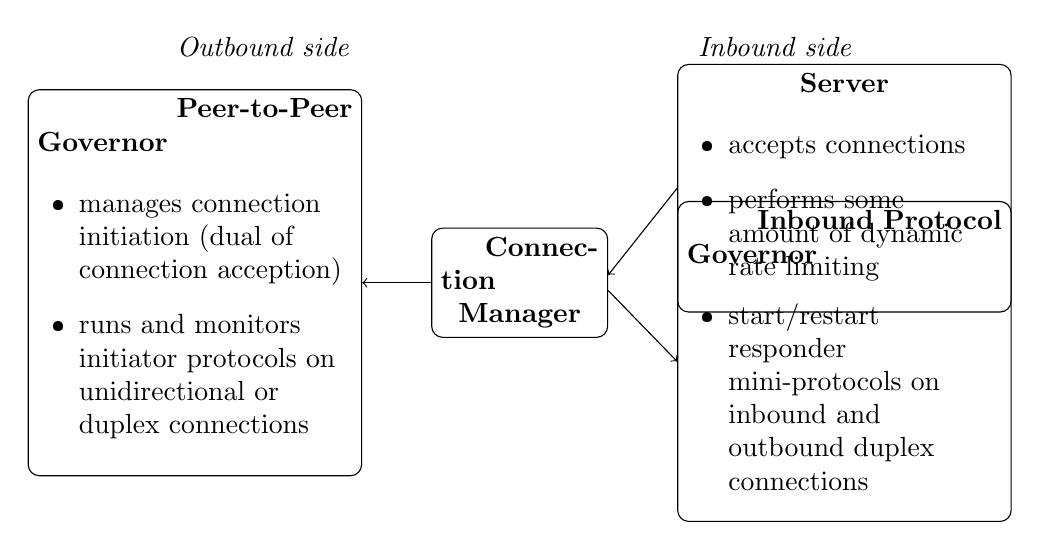
\begin{tikzpicture}
    \node at (-3.25, 0)  {\textit{Outbound side}};
    \node at ( 3.25, 0)  {\textit{Inbound side}};

    \node[rounded corners, rectangle, draw, minimum height=3cm,anchor=east, text width=4cm] (p2p_governor) at (\xa, -3)
     {
       \hfil\textbf{Peer-to-Peer Governor}\hfil\\
       \setlength{\leftmargini}{15pt}
       \begin{itemize}
        \item manages connection initiation (dual of connection acception)
        \item runs and monitors initiator protocols on unidirectional or duplex connections
      \end{itemize}
      \vspace{5pt}
      };

    \node[rounded corners, rectangle, draw, anchor=west, text width=4cm] (server) at (\xb, -1.80)
      {
        \hfill{\textbf{Server}}\hfill
        \vspace{0.2em}
        \setlength{\leftmargini}{15pt}
        \begin{itemize}
          \item accepts connections
          \item performs some amount of dynamic rate limiting
        \end{itemize}
        \vspace{5pt}
      };

    \node[rounded corners, rectangle, draw, anchor=west, text width=4cm] (inbound_governor) at (\xb, -4)
      {
        \hfill{\textbf{Inbound Protocol Governor}}\hfill
        \vspace{0.2em}
        \setlength{\leftmargini}{15pt}
        \begin{itemize}
          \item start/restart responder mini-protocols on inbound and
            outbound duplex connections
        \end{itemize}
        \vspace{5pt}
      };

    \node[rounded corners, rectangle, draw, minimum height=1cm, text width=2cm] (connection_manager) at (0, -3)
      {
        \hfil\textbf{Connection}\hfil\\
        \hfil\textbf{Manager}\hfil
      };

    \draw[<-] (p2p_governor)           -- (connection_manager);
    \draw[->] (server.west)            -- (connection_manager.5);
    \draw[->] (connection_manager.355) -- (inbound_governor.west);
  \end{tikzpicture}
  \caption{3 main components}
  \label{tik:components}
\end{figure}

One simple illustration of how these 3 components interact together:

\begin{itemize}
    \item Server accepts a connection;
    \item Server registers that connection to the connection manager (which puts the
      connection in \UnnegotiatedStateIn{});
    \item Assuming the handshake was successful, the connection is put in
      \InboundIdleStateDup{};
    \item The remote end transitions the local node to warm (using the connection) within expected timeout;
    \item IPG (Inbound Protocol Governor) notifies the \Connmngr{} about this state
      change, via \texttt{promotedToWarmRemote}. Now the connection is
      in \InboundStateDup{};
    \item \Connmngr{} is asked for an outbound connection to that peer (by the \ptopgov{}), it notices
      that it already has a connection with that peer in \InboundStateDup{}, so it gives
      that connection to \ptopgov{} and updates its state to \DuplexState{}.
\end{itemize}

You can find more information about the possible different connection states in section
\ref{sec:connection-state}.

\begin{figure}
    \centering
    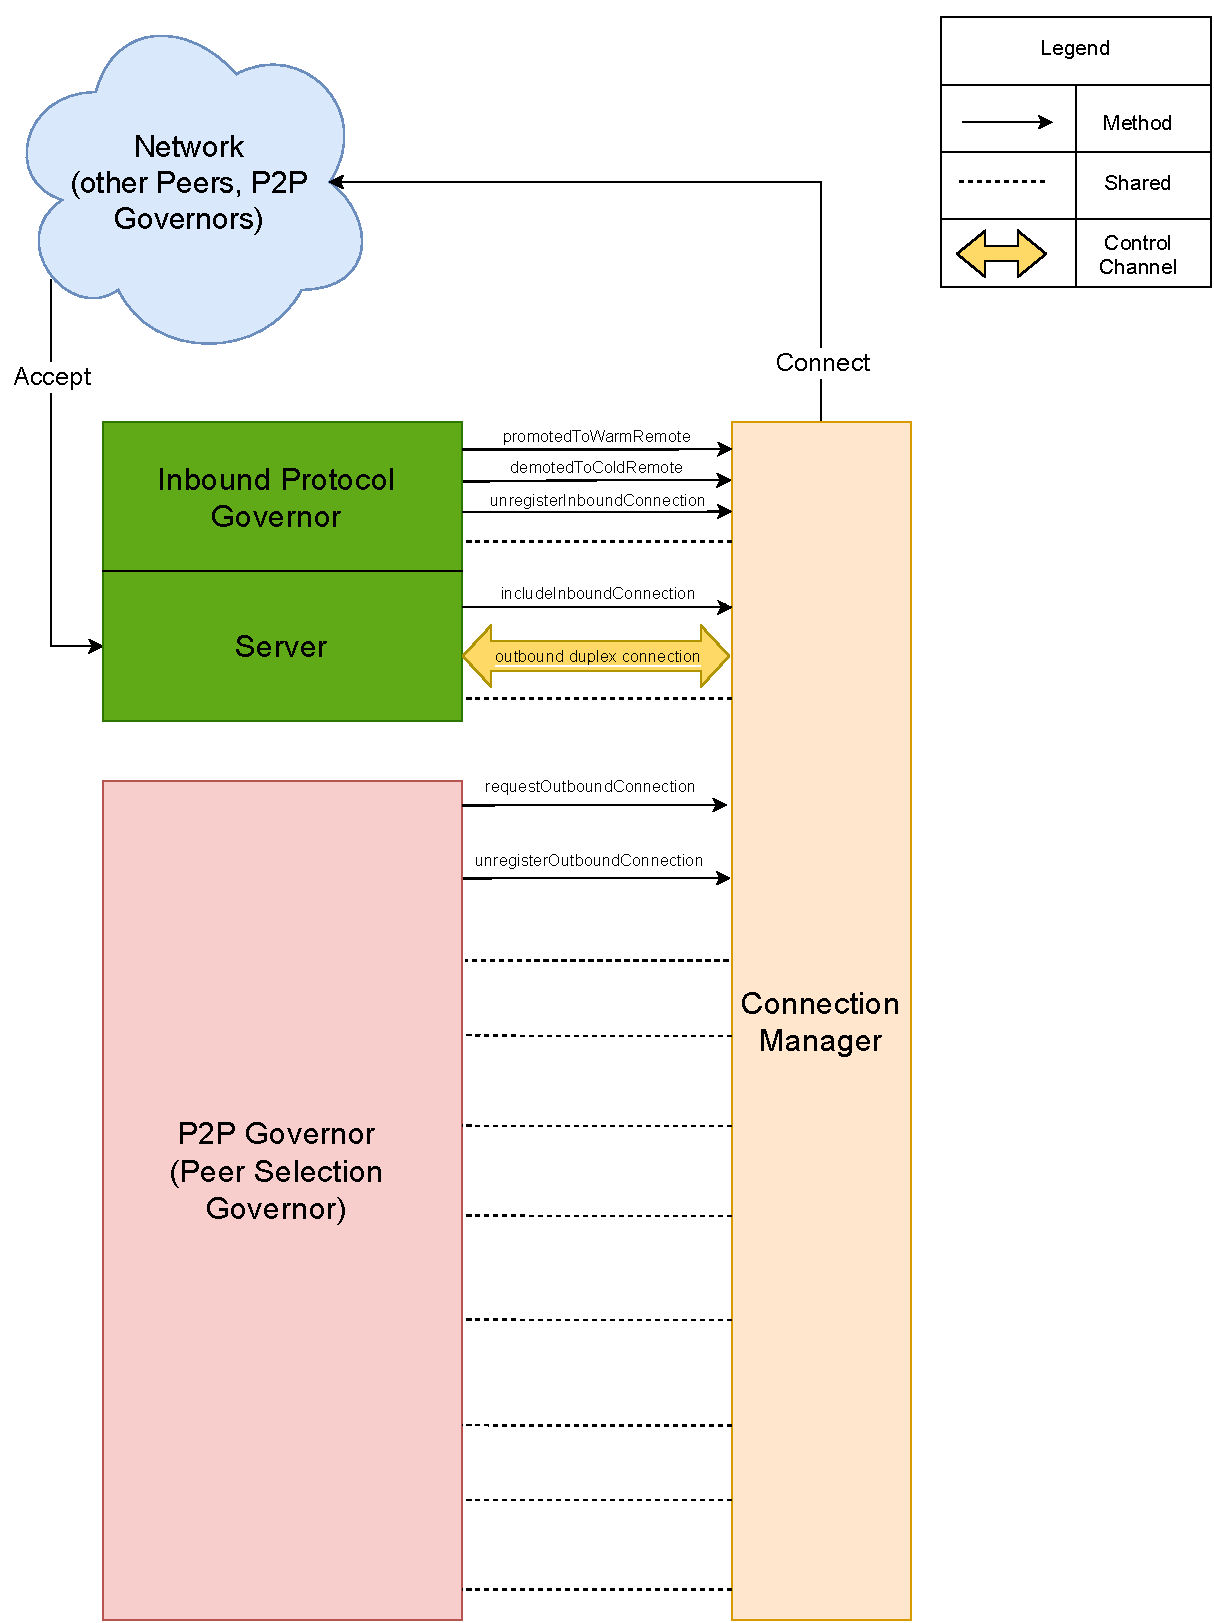
\includegraphics[width=\linewidth]{figure/ConnectionManagerInteractions.pdf}
    \caption{High-level architecture of how the 3 components interact}
    \label{fig:high-level-arch}
\end{figure}

Figure \ref{fig:high-level-arch} shows the high-level architecture of how the 3 components mentioned interact
with each other. A single \Connmngr{} is shared between the \emph{Server} and \ptopgov{},
where, in case of an \emph{Outbound Duplex} connection is negotiated, the \emph{Server} is
notified via a control channel. Although in this document we will use Server and IPG
interchangeably, it is worth to keep them separate concepts for possible future
developments.

\section{Connection Manager}

\subsection{Overview}

\Connmngr{} is a lower-level component responsible for managing connections and its
resources. Its responsibilities consist of:

\begin{itemize}
    \item Tracking each connection, in order to keep an eye on the bounded resources;
    \item Starting new connections, negotiating if the connection should be
      \emph{full-duplex} or \emph{half-duplex}, through the \emph{Connection Handler};
    \item Be aware of \warm{}/\hot{} transitions, in order to try and reuse already established
      connections;
    \item Negotiating which direction, which mini-protocol is going to run
      (Client $\rightarrow$ Server, Server$\rightarrow$Client, or both);
    \item Taking care of a particularity of TCP connection termination (lingering
      connections).
\end{itemize}

The \Connmngr{} creates and records accepted connections and keeps track of their state
as negotiations, for the connection and start/stop mini-protocols, are made. There's an
\emph{internal state machine} that helps the \Connmngr{} keep track of the state of each
connection, and help it make decisions when it comes to resource management and
connection reusing.

The \emph{Connection Handler} drives through handshake negotiation and starts the multiplexer. The
outcome of the handshake negotiation is:

\begin{itemize}
    \item the negotiated version of the protocol
    \item negotiated parameters, which includes the mode in which the connection will be
      run (\texttt{InitiatorOnlyMode}, \texttt{ResponderOnlyMode},\\
      \texttt{InitiatorAndResponderMode} - the first two are \emph{half-duplex}, the last
      one is \emph{full-duplex} mode)
    \item Handshake might error
\end{itemize}

\begin{figure}
    \centering
    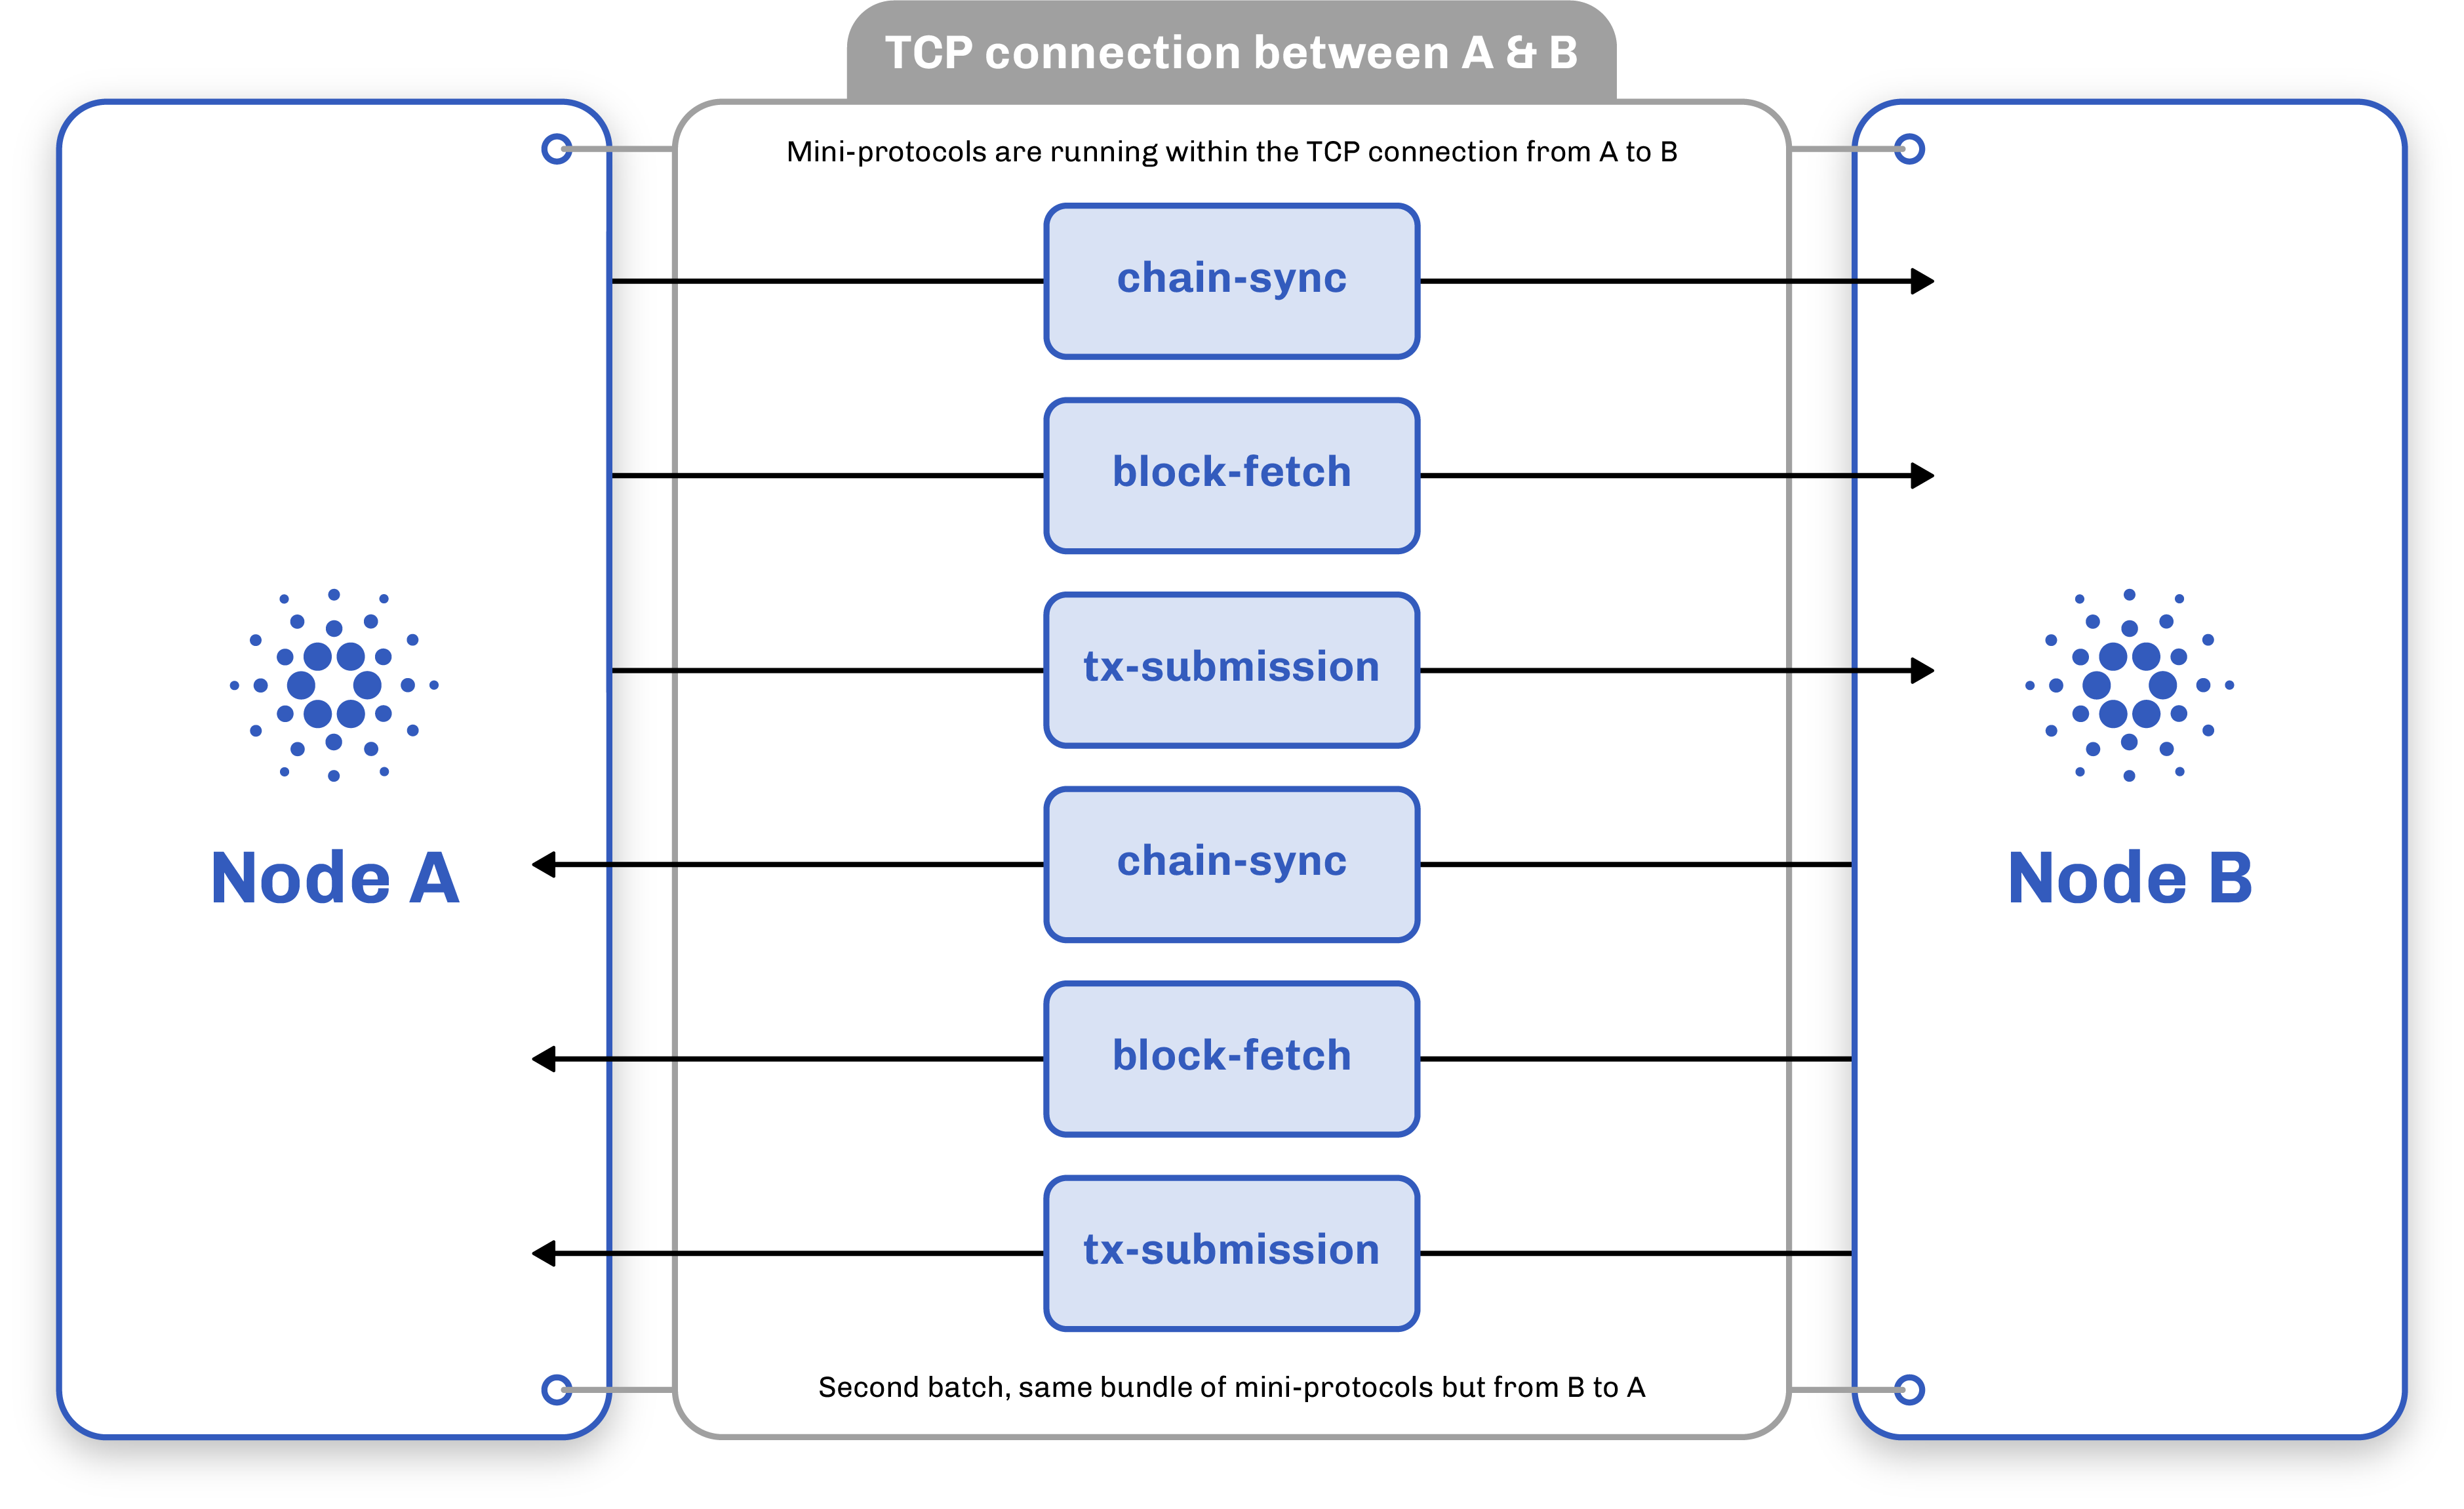
\includegraphics[width=\linewidth]{figure/node-to-node-ipc.png}
    \caption{Duplex connection running severall mini-protocols}
    \label{fig:protocol-diagram}
\end{figure}

The \emph{Connection Handler} notifies the \Connmngr{} about the result of a negotiation, which
triggers a state transition. If we can run the connection in full-duplex mode,
then it is possible to run the bundles of mini-protocols in both directions, and otherwise only in one direction.
So, Figure \ref{fig:protocol-diagram} shows $6$ mini protocols running, $3$ in each direction.
If we negotiated only a unidirectional connection, then we'd only be running $3$
(with the direction being based on which peer established the connection).

From the point of view of the \connmngr{}, it only
matters whether an \emph{unidirectional} or \emph{duplex} connection was negotiated.
Unidirectional connections, are the ones which run either the initiator or responder
side of mini-protocols, exclusively, while duplex connections can run either or
both initiator and responder protocols. Note that in the outbound direction (initiator side),
it is the \ptopgov{} responsibility to decide which set of mini-protocols:
\established{}, \warm{} or \hot{}, are running. On the inbound side (responder
mini-protocols), we have no choice but to run all of them.

The \connmngr{} should only be run in two \texttt{MuxMode}s:

\begin{itemize}
  \item \texttt{ResponderMode} or
  \item \texttt{InitiatorAndResponderMode}
\end{itemize}

\noindent, the \texttt{InitiatorMode} is not allowed, since that mode is reserved for
special leaf nodes in the network (such as the blockchain explorer, for example) and it doesn't make
sense to run a node-to-client client side.

The duplex mode: \texttt{InitiatorAndResponderMode} is useful for managing
connection with external nodes (\textit{node-to-node protocol}), while
\texttt{ResponderMode} is useful for running a server which responds to local
connections (server side of \textit{node-to-client protocol}).


\Connmngr{} can use at most one \ipvfour{} and at most one \ipvsix{}
address. It will bind to the correct address depending on the remote address
type (\ipvfour{}/\ipvsix{}).

In this specification we will often need to speak about two nodes communicating
via a \TCP{} connection.  We will often call them local and remote ends of the
connection or local \slash{} remote nodes; we will usually take the
perspective of the local node.


\subsection{Types} % Not sure about this naming

\Connmngr{} exposes two methods to register a connection:

\begin{lstlisting}
data Connected peerAddr handle handleError
  -- | We are connected and mux is running.
  = Connected    !(ConnectionId peerAddr) !handle

  -- | There was an error during handshake negotiation.
  | Disconnected !(ConnectionId peerAddr) !(Maybe handleError)

-- | Include outbound connection into 'ConnectionManager'.

--   This executes:
--
-- * \(Reserve\) to \(Negotiated^{*}_{Outbound}\) transitions
-- * \(PromotedToWarm^{Duplex}_{Local}\) transition
-- * \(Awake^{Duplex}_{Local}\) transition
requestOutboundConnection
  *'$\coloncolon$'* HasInitiator muxMode ~ True
  *'$\Rightarrow$'* ConnectionManager muxMode socket peerAddr handle handleError m
  *'$\rightarrow$'* peerAddr *'$\rightarrow$'* m (Connected peerAddr handle handleError)

-- | Include an inbound connection into 'ConnectionManager'.

--   This executes:
--
-- * \(Accepted\) \/ \(Overwritten\) to \(Negotiated^{*}_{Inbound}\) transitions
includeInboundConnection
  *'$\coloncolon$'* HasResponder muxMode ~ True
  *'$\Rightarrow$'* ConnectionManager muxMode socket peerAddr handle handleError m
  *'$\rightarrow$'* socket *'$\rightarrow$'* peerAddr *'$\rightarrow$'* m (Connected peerAddr handle handleError)
\end{lstlisting}

The first one asks the \connmngr{} to either connect to an outbound peer or, if
possible, reuse a duplex connection. The other one allows to register an
inbound connection, which was \texttt{accepted}. Both methods are blocking
operations and return either an error (handshake negotiation error or
a multiplexer error) or a handle to a \textit{negotiated} connection.

Other methods which are discussed in this specification:

\begin{lstlisting}
-- | Custom either type for result of various methods.
data OperationResult a
    = UnsupportedState !InState
    | OperationSuccess a

-- | Enumeration of states, used for reporting; constructors elided from this
-- specification.
data InState

-- | Unregister an outbound connection.
--
--   This executes:
--
-- * \(DemotedToCold^{*}_{Local}\) transitions
unregisterOutboundConnection
  *'$\coloncolon$'* HasInitiator muxMode ~ True
  *'$\Rightarrow$'* ConnectionManager muxMode socket peerAddr handle handleError m
  *'$\rightarrow$'* peerAddr *'$\rightarrow$'* m (OperationResult ())

-- | Notify the 'ConnectionManager' that a remote end promoted us to a
-- /warm peer/.
--
-- This executes:
--
-- * \(PromotedToWarm^{Duplex}_{Remote}\) transition,
-- * \(Awake^{*}_{Remote}\) transition.
promotedToWarmRemote
  *'$\coloncolon$'* HasInitiator muxMode ~ True
  *'$\Rightarrow$'* ConnectionManager muxMode socket peerAddr handle handleError m
  *'$\rightarrow$'* peerAddr *'$\rightarrow$'* m (OperationResult InState)

-- | Notify the 'ConnectionManager' that a remote end demoted us to a /cold
-- peer/.
--
-- This executes:
--
-- * \(DemotedToCold^{*}_{Remote}\) transition.
demotedToColdRemote
  *'$\coloncolon$'* HasResponder muxMode ~ True
  *'$\Rightarrow$'* ConnectionManager muxMode socket peerAddr handle handleError m
  *'$\rightarrow$'* peerAddr -> m (OperationResult InState)

-- | Unregister outbound connection. Returns if the operation was successul.
--
-- This executes:
--
-- * \(Commit*{*}\) transition
-- * \(TimeoutExpired\) transition
unregisterInboundConnection
  *'$\coloncolon$'* HasResponder muxMode ~ True
  *'$\Rightarrow$'* ConnectionManager muxMode socket peerAddr handle handleError m
  *'$\rightarrow$'* peerAddr *'$\rightarrow$'* m (OperationResult DemotedToColdRemoteTr)

-- | Number of connections tracked by the server.
numberOfConnections
  *'$\coloncolon$'* HasResponder muxMode ~ True
  *'$\Rightarrow$'* ConnectionManager muxMode socket peerAddr handle handleError m
  *'$\rightarrow$'* STM m Int
\end{lstlisting}

\subsection{Connection states}\label{sec:connection-state}

Each connection is either initiated by \texttt{Inbound} or \texttt{Outbound} side.

\begin{lstlisting}
data Provenance
  = Inbound
  | Outbound
\end{lstlisting}
Each connection negotiates \texttt{dataFlow}:
\begin{lstlisting}
data DataFlow
  = Unidirectional
  | Duplex
\end{lstlisting}

In \texttt{Unidirectional} data flow, the connection is only used in one direction:
the outbound side runs initiator side of mini-protocols, the inbound side runs
responders; in \texttt{Duplex} mode, both inbound and outbound side runs
initiator and responder side of each mini-protocol. Negotiation of
\texttt{DataFlow} is done by the handshake protocol, the final result depends
on two factors: negotiated version and \texttt{InitiatorOnly} flag which is
announced through handshake. Each connection can be in one of the following
states:

\begin{lstlisting}
data ConnectionState
  -- Connection manger is about to connect to a peer.
  = ReservedOutboundState

  -- Connected to a peer, handshake negotiation is ongoing.
  | UnnegotiatedState Provenance

  -- Outbound connection, inbound idle timeout is ticking.
  | OutboundState*'$^\tau$'* DataFlow

  -- Outbound connection, inbound idle timeout expired.
  | OutboundState DataFlow

  -- Inbound connection, but not yet used.
  | InboundIdleState*'$^\tau$'* DataFlow

  -- Active inbound connection.
  | InboundState DataFlow

  -- Connection runs in duplex mode: either outbound connection negotiated
  -- 'Duplex' data flow, or 'InboundState Duplex' was reused.
  | DuplexState

  -- Connection manager is about to close (reset) the connection, before it
  -- will do that it will put the connection in 'OutboundIdleState' and start
  -- a timeout.
  | OutboundIdleState*'$^\tau$'*

  -- Connection has terminated; socket is closed, thread running the
  -- connection is killed.  For some delay (`TIME_WAIT`) the connection is kept
  -- in this state until the kernel releases all the resources.
  | TerminatingState

  -- Connection is forgotten.
  | TerminatedState
\end{lstlisting}

The above type is a simplified version of what is implemented. The real
implementation tracks more detail, e.g. connection id (the quadruple of ip
addresses and ports), multiplexer handle, thread id etc., which we do not need
to take care in this specification. The rule of thumb is that all states that
have some kind of timeout should be annotated with a $\tau$. In these cases we
are waiting for any message that would indicate a \warm{} or \hot{} transition.
If that does not happen within a timeout we will close the connection.

In this specification we represent \OutboundStateUniTau{} which is not used,
the implementation avoids this constructor, for the same reasons that were given above,
regarding \texttt{InitiatorMode}.

\begin{figure}[p]
  {\begin{tikzpicture}[scale=0.66]
    \node                                     (init)                       at ( 2,   2)     {\small\InitialState};
    \node[outbound_state]                     (ReservedOutboundState)      at ( 0,-0.25)    {\small\ReservedOutboundState};
    \node[outbound_state,anchor=east]         (UnnegotiatedStateOut)       at (-1,  -3)     {\small\UnnegotiatedStateOut};
    \node[inbound_state]                      (UnnegotiatedStateIn)        at ( 5.5, -3)    {\small\UnnegotiatedStateIn};
    \node[inbound_outbound_state,anchor=west] (InboundIdleStateDup)        at ( 1, -6.0)    {\small\InboundIdleStateDup};
    \node[inbound_state,anchor=west]          (InboundIdleStateUni)        at ( 5, -8)      {\small\InboundIdleStateUni};
    \node[outbound_state,anchor=east]         (OutboundStateUni)           at (-2, -7.5)    {\small\OutboundStateUni};
    \node[inbound_outbound_state,anchor=east] (OutboundStateDupTau)        at (-1, -10.5)   {\small\OutboundStateDupTau};
    \node[inbound_outbound_state,anchor=east] (OutboundStateDup)           at (-1,  -14.0)  {\small\OutboundStateDupP};
    \node[inbound_state,anchor=west]          (InboundStateUni)            at ( 5, -16.0)   {\small\InboundStateUni};
    \node[inbound_outbound_state,anchor=west] (InboundStateDup)            at ( 1,  -13.5)  {\small\InboundStateDup};
    \node[inbound_outbound_state]             (DuplexState)                at (-1.5, -21.5) {\small\DuplexState};
    \node[inbound_outbound_state]             (OutboundIdleStateDup)       at ( 5,  -23)    {\small\OutboundIdleStateDup};
    \node[outbound_state]                     (OutboundIdleStateUni)       at (-5,  -24.5)  {\small\OutboundIdleStateUni};
    \node[inbound_outbound_state]             (TerminatingState)           at ( 3,  -27)    {\small\TerminatingState};
    \node[inbound_outbound_state]             (TerminatedState)            at ( 3,  -30)    {\small\TerminatedState};


    \draw[->] (init) -- node[fill=white,pos=0.425,above left]{\small\Reserve}                                          (ReservedOutboundState);
    \draw[->] (init) to [out=310, in=90] node[fill=white, above right]{\small\Accepted}                                (UnnegotiatedStateIn.30);

    \draw[->] (ReservedOutboundState)          -- node[fill=white,above left] {\small\Connected}                       (UnnegotiatedStateOut);
    \draw[->] (ReservedOutboundState)          -- node[fill=white,above right] {\small\Overwritten}                    (UnnegotiatedStateIn);

    \draw[->] (UnnegotiatedStateOut)           -- node[fill=white,left=-42pt] {\small\NegotiatedUniOut}                (OutboundStateUni.165);
    \draw[->] (UnnegotiatedStateOut.340)       to [out=-60, in=90]
                                               node[fill=white,right=-30pt,pos=0.23]{\small\NegotiatedDupOut}          (OutboundStateDupTau.13);

    \draw[->]         (UnnegotiatedStateIn)    -- node[fill=white,left=-12pt]{\small\NegotiatedDupIn}                  (InboundIdleStateDup.150);
    \draw[->]         (UnnegotiatedStateIn)    -- node[fill=white,pos=0.35,right=-28pt]{\small\NegotiatedUniIn}        (InboundIdleStateUni.60);

    \draw[->]         (InboundIdleStateUni.320) to [out=-90,in=40]
                                                node[fill=white,pos=0.5,rotate=70,left=-15pt]{\small\CommitUniRem}     (TerminatingState.0);
    \draw[->, dashed] (InboundStateUni.10)      -- node[pos=0.3,fill=white,right=-45pt]{\small\DemotedToColdUniRem}    (InboundIdleStateUni.350);
    \draw[->]         (InboundIdleStateDup.195) -- node[fill=white,pos=0.4]{\small\AwakeDupLoc}                        (OutboundStateDupTau.10);

    \draw[->, dashed] (InboundIdleStateDup.200) -- node[fill=white,pos=0.65]{\small\AwakeDupRem}                       (InboundStateDup.160);
    \draw[->]         (OutboundStateDupTau.150) to [out=90,in=-170]
                                                node[fill=white,pos=0.10,left=-56pt]{\small\DemotedToColdDupLoc}       (InboundIdleStateDup.180);
    \draw[->]         (OutboundStateDup.192)    to [out=-90,in=180,looseness=2]
                                                node[fill=white,rotate=90,pos=0.2]{\small\DemotedToColdDupLoc}         (OutboundIdleStateDup.180);
    \draw[->]         (OutboundStateDupTau.192) --
                                                node[fill=white] {\small\TimeoutExpired}
                                                (OutboundStateDup.168);
    \draw[->]         (InboundStateDup)         to [out=-110,in=40]
                                                node[pos=0.9,right=20pt,rotate=70]{\footnotesize\PromotedToWarmDupLoc}     (DuplexState.10);
    \draw[->, dashed] (OutboundIdleStateDup.60) to [out=90, in=270]
                                                node[fill=white,rotate=90,pos=0.6,below=30pt]{\footnotesize\AwakeDupRem}   (InboundStateDup.345);
    \draw[->]         (DuplexState)             to [out=50,in=220]
                                                node[fill=white,pos=0.90,left=24pt,rotate=65]{\small\DemotedToColdDupLoc}  (InboundStateDup);
    \draw[->, dashed] (DuplexState.155)         to [out=90,in=-40]
                                                node[fill=white,right=10pt,pos=0.01,rotate=80]{\small\DemotedToColdDupRem} (OutboundStateDupTau);

    \draw[dashed] (OutboundStateDupTau)         -- (OutboundStateDup.south);
    \filldraw (OutboundStateDupTau.south) circle [radius=3pt];
    \filldraw (OutboundStateDup.south)    circle [radius=3pt];
    \draw[->, dashed] (OutboundStateDup)        to [out=-90,in=180]
                                                node[left,pos=0.05,left=10pt,rotate=80]{\small\PromotedToWarmDupRem}  (DuplexState);

    \draw[->]         (InboundIdleStateDup.270) to [out=-80,in=80]
                                                      node[fill=white,pos=0.5,left=-10pt,rotate=80]{\small\CommitDupRem} (TerminatingState.155);
    \draw[->, dashed] (InboundIdleStateUni.200) -- node[fill=white,right=-15pt]{\small\AwakeUniRem}                   (InboundStateUni.160);
    \draw[->, dashed] (InboundStateDup.15)      -- node[fill=white,left=-75pt,pos=0.5]{\small\DemotedToColdDupRem}    (InboundIdleStateDup.345);
    \draw[->]         (OutboundStateUni.190)    to [out=270, in=90,pos=0.23,looseness=2]
                                                node[fill=white,rotate=88,pos=0.3]{\small\DemotedToColdUniLoc}        (OutboundIdleStateUni.173);

    \draw[->]         (OutboundIdleStateUni)       to [out=300, in=180] node[fill=white,below left]{\CommitUniLoc}         (TerminatingState.180);
    \draw[->]         (OutboundIdleStateDup.280)   -- node[fill=white,pos=.4]{\CommitDupLoc}                          (TerminatingState.40);
    \draw[->]         (TerminatingState)           -- node[left]{\Terminate}                                          (TerminatedState);
  \end{tikzpicture}}
  \caption{\textit{Outbound} (blue \& violet) and \textit{inbound} (green \&
  violet) connection states and allowed transitions.}
  \label{fig:statediagram}
\end{figure}

Figure~\ref{fig:statediagram} shows all the transitions between
\texttt{ConnectionState}s. Blue and Violet states represent states of
an \textit{Outbound} connection, Green and Violet states represent states of an
\textit{Inbound} connection. Dashed arrows indicate asynchronous
transitions that are triggered, either by a remote node or by the connection
manager itself.

Note that the vertical symmetry in the graph corresponds to local vs remote
state of the connection, see table~\ref{table:symmetry}. The symmetry is only
broken by \InboundIdleStateAny{} which does not have a corresponding
local equivalent. This is simply because, locally we immediately know when we
start initiator-protocols, and the implementation is supposed to do that
promptly. This however, cannot be assumed about the inbound side.

\begin{table}[h]
  \begin{tabular}[h]{l|l}
    \textit{local connection state} & \textit{remote connection state} \\ [0.3em]
    \hline \\
    \UnnegotiatedStateOut{}         & \UnnegotiatedStateIn{}           \\ [0.2em]
    \OutboundIdleStateAny{}         & \InboundIdleStateAny{}           \\ [0.2em]
    \OutboundStateAny{}             & \InboundStateAny{}               \\ [0.2em]
    \OutboundStateAnyTau{}          & \InboundStateAny{}               \\ [0.2em]
    \InboundStateAny{}              & \OutboundStateAny{}              \\ [0.2em]
    \DuplexState{}                  & \DuplexState{}                   \\ [0.2em]
  \end{tabular}
  \caption{Symmetry between local and remote states}
  \label{table:symmetry}
\end{table}

Another symmetry that we tried to preserve is between \texttt{Unidirectional}
and \texttt{Duplex} connections. The \texttt{Duplex} side is considerably more
complex as it includes interaction between \texttt{Inbound} and
\texttt{Outbound} connections (in the sense that inbound connection can migrate
to outbound only and vice versa). However, the state machine for an inbound
only connection is the same whether it is \texttt{Duplex} or
\texttt{Unidirectional}, see Figure~\ref{fig:statediagram-inbound-only}.
A \connmngr{} running in \texttt{ResponderMode} will use this state
machine.

For \textit{node-to-client} server it will be even simpler, as there
we only allow for unidirectional connections. Nevertheless, this symmetry
simplifies the implementation.

\begin{figure}[p]
  {\begin{tikzpicture}[scale=0.66]
    \node                                     (init)                       at ( 2,   2)   {\small\InitialState};
    \node[inbound_outbound_state]             (ReservedOutboundState)      at ( 0,-0.25)  {\small\ReservedOutboundState};
    \node[inbound_outbound_state]             (UnnegotiatedStateIn)        at ( 5.5, -3)  {\small\UnnegotiatedStateIn};
    \node[inbound_outbound_state,anchor=west] (InboundIdleStateDup)        at ( 0, -7.0)  {\small\InboundIdleStateDup};
    \node[inbound_state,anchor=west]          (InboundIdleStateUni)        at ( 8, -7)    {\small\InboundIdleStateUni};
    \node[inbound_state,anchor=west]          (InboundStateUni)            at ( 7.5, -12) {\small\InboundStateUni};
    \node[inbound_outbound_state,anchor=west] (InboundStateDup)            at ( 0,  -12)  {\small\InboundStateDup};
    \node[inbound_outbound_state]             (TerminatingState)           at ( 6,  -16)  {\small\TerminatingState};
    \node[inbound_outbound_state]             (TerminatedState)            at ( 6,  -19)  {\small\TerminatedState};


    \draw[->] (init) -- node[fill=white,pos=0.425,above left]{\small\Reserve}                                      (ReservedOutboundState);
    \draw[->] (init) to [out=310, in=90] node[fill=white, above right]{\small\Accepted}                            (UnnegotiatedStateIn.30);

    \draw[->] (ReservedOutboundState)          -- node[fill=white,above right] {\small\Overwritten}                (UnnegotiatedStateIn);

    \draw[->]         (UnnegotiatedStateIn)  -- node[fill=white,left=-12pt]{\small\NegotiatedDupIn}                (InboundIdleStateDup.150);
    \draw[->]         (UnnegotiatedStateIn)  -- node[fill=white,pos=0.35,right=-28pt]{\small\NegotiatedUniIn}      (InboundIdleStateUni.60);
    \draw[->, dashed] (InboundIdleStateUni.347) -- node[fill=white,pos=0.35,right=-15pt]{\small\AwakeUniRem}       (InboundStateUni.15);


    \draw[->, dashed] (InboundIdleStateDup.200) -- node[fill=white,pos=0.65]{\small\AwakeDupRem}                   (InboundStateDup.160);

    \draw[->]         (InboundIdleStateDup.270) to [out=-80,in=110]
                                                      node[fill=white,pos=0.8]{\small\CommitDupRem}                (TerminatingState.170);
    \draw[->]         (InboundIdleStateUni.320) to [out=-90,in=50]
                                                      node[fill=white,pos=0.8]{\small\CommitUniRem}                (TerminatingState.10);
    \draw[->, dashed] (InboundStateDup.15)      -- node[fill=white,left=-85pt,pos=0.6]{\small\DemotedToColdDupRem} (InboundIdleStateDup.345);
    \draw[->, dashed] (InboundStateUni.165)     -- node[pos=0.3,fill=white]{\small\DemotedToColdUniRem}            (InboundIdleStateUni.200);
    % \draw[->]         (OutboundStateUni.195)    to [out=270, in=180,pos=0.23,looseness=2]
                                                      % node[right=12pt,rotate=88,pos=0.3]{\small\DemotedToColdUniLoc}  (TerminatingState.175);

\def\OutboundStateDup{\texttt{OutboundState Duplex}}
    \draw[->] (TerminatingState) -- node[fill=white]{\Terminate} (TerminatedState);
  \end{tikzpicture}}
  \caption{Sub-graph of inbound states.}
  \label{fig:statediagram-inbound-only}
\end{figure}


\subsection{Transitions}


\subsubsection{\Reserve{}}
When \connmngr{} is asked for an outbound connection, it reserves a slot
in its state for that connection.  If any other thread asks for the same
outbound connection, the \connmngr{} will raise an exception in that thread.
Reservation is done to guarantee exclusiveness for state transitions to
a single outbound thread.

\subsubsection{\Connected{}}
This transition is executed once an outbound connection successfully performed the
\texttt{connect} system call.

\subsubsection{\Accepted{} and \Overwritten{}}
Transition driven by the \texttt{accept} system call. Once it returns, the
\connmngr{} might either not know about such connection or, there might be one
in \ReservedOutboundState{}. The \Accepted{} transition represents the former
situation, while the latter is captured by the \Overwritten{} transition.

Let us note that if \Overwritten{} transition happened, then on the outbound
side, the scheduled \texttt{connect} call will fail. In this case the
\ptopgov{} will recover, putting the peer in a queue of failed peers, and
will either try to connect to another peer, or reconnect to that peer after some
time, in which case it would re-use the accepted connection (assuming that
a duplex connection was negotiated).

\subsubsection{\NegotiatedUniOut{} and \NegotiatedDupOut{}}
Once an outbound connection has been negotiated one of \NegotiatedUniOut{} or
\NegotiatedDupOut{} transition is performed, depending on the result of handshake
negotiation. Duplex connections are negotiated only for node-to-node protocol
versions higher than \texttt{NodeToNodeV\_7}\todoimpl{the exact version number
might change} and neither side declared that it is an \emph{initiator} only.

If duplex outbound connection was negotiated, the \connmngr{} needs to ask the
\inbgov{} to start and monitor responder mini-protocols on the outbound
connection.

\begin{detail}
This transition is done by the \texttt{requestOutboundConnection}.
\end{detail}


\subsubsection{\NegotiatedUniIn{} and \NegotiatedDupIn{}}
This transition is performed once handshake negotiated an unidirectional or
duplex connection on an inbound connection.

For \NegotiatedUniIn{}, \NegotiatedDupIn{}, \NegotiatedDupOut{}
transitions, the \textit{inbound protocol governor} will restart all responder
mini-protocols (for all \established{}, \warm{} and \hot{} groups of
mini-protocols) and keep monitoring them.

\begin{detail}
This transition is done by the \texttt{includeInboundConnection}.
\end{detail}

\begin{detail}
  Whenever a mini-protocol terminates it is immediately restarted using
  an on-demand strategy. All \textit{node-to-node} protocols have initial agency
  on the client side, hence restarting them on-demand does not send any
  message.
\end{detail}


\subsubsection{\AwakeDupLoc{}, \AwakeDupRem{} and \AwakeUniRem{}}
All the awake transitions start either at \InboundIdleStateAny{}, the
\AwakeDupRem{} can also be triggered on \OutboundIdleStateDup{}.

\begin{detail}
  \AwakeDupLoc{} transition is done by \texttt{requestOutboundConnection} on
  the request of \ptopgov{}, while \AwakeDupRem{} and \AwakeUniRem{} are
  triggered by incoming traffic on any of responder mini-protocols (asynchronously if
  detected any \warm{}/\hot{} transition).
\end{detail}


\subsubsection{\CommitUniRem{}, \CommitDupRem{}}\label{sec:tr_commit}
Both commit transitions happen after \textit{protocol idle timeout} of
inactivity (as the \TimeoutExpired{} transition does). They transition to
\TerminatingState{} (closing the bearer). For duplex connections a normal
shutdown procedure goes through \InboundIdleStateDup{}
via \CommitDupRem{} - which gave the name to this transition.

These transitions are triggered by inactivity of responder mini-protocols. They
both protect against a client that connects but never sends any data through
the bearer; also, as part of a termination sequence, it is protecting us from
shutting down a connection which is transitioning between \warm{} and \hot{}
states.

Both commit transitions:
\begin{itemize}
  \item \CommitDupRem{}
  \item \CommitUniRem{}
\end{itemize}
need to detect idleness during time interval (which we call: \text{protocol
idle timeout}). If during this time frame inbound traffic on any responder
mini-protocol is detected, one of the \AwakeDupRem{} or \AwakeUniRem{}
transition is performed. The idleness detection might also be interrupted by
the local \AwakeDupLoc{} transition.

\begin{detail}
  These transitions can be triggered by \texttt{unregisterInboundConnection} and
  \texttt{unregisterOutboundConnection} (both are non-blocking), but the
  stateful idleness detection during \textit{protocol idle timeout} is
  implemented by the server.

  The implementation is relaying on two properties:
  \begin{itemize}
    \item the multiplexer being able to start mini-protocols on-demand, which
      allows us to restart a mini-protocol as soon as it returns, without
      disturbing idleness detection;
    \item the initial agency for any mini-protocol is on the client.
  \end{itemize}
\end{detail}

\begin{detail}
  Whenever an outbound connection is requested, we notify the server about
  a new connection.  We do that also when the connection manager hands over an
  existing connection.  If \inbgov{} is already tracking that connection,
  we need to make sure that
  \begin{itemize}
    \item \inbgov{} preserves its internal state of that connection;
    \item \inbgov{} does not starts mini-protocols, as they are already running
      (we restart responders as soon as the stop, using the on-demand
      strategy).
  \end{itemize}
\end{detail}


\subsubsection{\DemotedToColdUniLoc{}, \DemotedToColdDupLoc{}}
This transitions is driven by the \ptopgov{} when it decides to demote the peer
to \cold{} state, its domain is \OutboundStateAny{} or \OutboundStateDupTau{}.
The target state is \OutboundIdleStateAny{} in which the connection manager
sets up a timeout.  When the timeout expires connection manager will do
\CommitAnyLoc{} transition, which will reset the connection.

\begin{detail}
This transition is done by \texttt{unregisterOutboundConnection}.
\end{detail}


\subsubsection{\DemotedToColdUniRem{}, \DemotedToColdDupRem{}}
Both transitions are edge-triggered, the connection manager is notified by the
\inbgov{} once it notices that all responders became idle. Detection of
idleness during \textit{protocol idle timeout} is done in a separate step which
is triggered immediately, see section~\ref{sec:tr_commit_rem} for details.

\begin{detail}
  Both transitions are done by \texttt{demotedToColdRemote}.
\end{detail}


\subsubsection{\PromotedToWarmDupLoc{}}
This transition is driven by the local \ptopgov{} when it promotes a \cold{} peer
to \warm{} state. \connmngr{} will provide a handle to an existing connection, so that
\ptopgov{} can drive its state.

\begin{detail}
This transition is done by \texttt{requestOutboundConnection}.
\end{detail}


\subsubsection{\TimeoutExpired{}}
This transition is triggered when the protocol idleness timeout expires while
the connection is in \OutboundStateDupTau{}. The server starts this timeout
when it triggers \DemotedToColdAnyRem{} transition. The connection manager
tracks the state of this timeout so we can decide if a connection in outbound
state can terminate or it needs to await for that timeout to expire.

\begin{detail}
  This transition is done by \texttt{unregisterInboundConnection}.
\end{detail}


\subsubsection{\PromotedToWarmDupRem{}}
This asynchronous transition is triggered by the remote peer.  The \inbgov{}
can notice it by observing multiplexer ingress side of running mini-protocols.
It then should notify the \connmngr{}.

\begin{detail}
  This transition is done by \texttt{promotedToWarmRemote}.

  The implementation relies on two properties:
  \begin{itemize}
    \item all initial states of node-to-node mini-protocols have client agency, i.e. the
      server expects an initial message;
    \item all mini-protocols are started using on-demand strategy, which allows
      to detect when a mini-protocol is brought to life by the multiplexer.
  \end{itemize}
\end{detail}


\subsubsection{\Prune{} transitions}
First let us note that a connection in \InboundStateDup{}, could have been
initiated by either side (Outbound or Inbound). This means that even though a node might have not
accepted any connection, it could end up serving peers and possibly go beyond
server hard limit, thus exceeding the number of file descriptors. This is
possible via the following path:
\begin{itemize}
  \item[] \Connected{},
  \item[] \NegotiatedDupOut{},
  \item[] \PromotedToWarmDupRem{},
  \item[] \DemotedToColdDupLoc{}
\end{itemize}

which leads from the initial state \InitialState{} to \InboundStateDup{}, the
same state in which accepted duplex connections end up. Even though the server
rate limits connections based on how many connections are in this state, we
could end up exceeding server hard limit.

To solve this problem, when a connection is transitioned from
\DuplexState{} to \InboundStateDup{} (via \DemotedToColdDupLoc{}) the
\connmngr{} will check if the server hard limit was exceeded. If that
happened, the \connmngr{} will reset an arbitrary connection (with some preference).

We prefer to reset an inbound connection rather than close an outbound
connection because from a systemic point of view, outbound connections are more
valuable than inbound ones. If we keep the number of \established{} peers to
be smaller than the server hard limit, with a right policy we should never need
to reset a connection in \DuplexState{}.

The \textit{inbound protocol governor} is in position to make an educated
decision about which connection to reset. Initially, we aim for a decision driven by
randomness, but other choices are possible\footnote{We can take into account
whether we are \hot{} to the remote end, or for how long we have been \hot{} to
to the remote node.} and the implementation should allow to easily extend the
initial choice.


\subsubsection{\CommitUniRem{}, \CommitDupRem{}}\label{sec:tr_commit_rem}
Both commit transitions happen after \textit{protocol idle timeout} of
inactivity (as the \TimeoutExpired{} transition does). They transition to
\TerminatingState{} (closing the bearer). For duplex connections a normal
shutdown procedure goes through \InboundIdleStateDup{}
via \CommitDupRem{} - which gave the name to this transition, or through
\OutboundIdleStateDup{} via \CommitDupLoc{} transition.

These transitions are triggered by inactivity of responder mini-protocols. They
both protect against a client that connects but never sends any data through
the bearer; also, as part of a termination sequence, it is protecting us from
shutting down a connection which is transitioning between \warm{} and \hot{}
states.

Both commit transitions:
\begin{itemize}
  \item \CommitDupRem{}
  \item \CommitUniRem{}
\end{itemize}

need to detect idleness during time interval (which we call: \text{protocol
idle timeout}). If during this time frame inbound traffic on any responder
mini-protocol is detected, one of the \AwakeDupRem{} or \AwakeUniRem{}
transition is performed. The idleness detection might also be interrupted by
the local \AwakeDupLoc{} transition.

\begin{detail}
  These transitions can be triggered by \texttt{unregisterInboundConnection} and
  \texttt{unregisterOutboundConnection} (both are non-blocking), but the
  stateful idleness detection during \textit{protocol idle timeout} is
  implemented by the \inbgov{}.  The implementation is relying on two
  properties:
  \begin{itemize}
    \item the multiplexer being able to start mini-protocols on-demand, which
      allows us to restart a mini-protocol as soon as it returns, without
      disturbing idleness detection;
    \item the initial agency for any mini-protocol is on the client.
  \end{itemize}
\end{detail}

\begin{detail}
  Whenever an outbound connection is requested, we notify the server about
  a new connection.  We do that also when the connection manager hands over an
  existing connection.  If \inbgov{} is already tracking that connection,
  we need to make sure that
  \begin{itemize}
    \item \inbgov{} preserves its internal state of that connection;
    \item \inbgov{} does not starts mini-protocols, as they are already running
      (we restart responders as soon as the stop, using the on-demand
      strategy).
  \end{itemize}
\end{detail}


\subsubsection{\CommitUniLoc{}, \CommitDupLoc{}}\label{sec:tr_commit_loc}
As previous two transitions, these also are trigged after \textit{protocol idle
timeout}, but this time are triggered on the outbound side.  These transition
will reset the connection, and the timeout make sure that the remote end will
be able to clear its ingress queue before the \TCP{} reset arrives.  For a more
detailed analysis see~\ref{sec:connection-close} section.


\subsubsection{\Terminate{}}
After a connection was closed, we keep it in \TerminatingState{} for the
duration of \textit{wait time timeout}.  When the timeout expires the
connection is forgotten.  \todo[inline]{Add a haddock link to \texttt{daTimeWaitTimeout}}


\subsection{Protocol errors}
If a mini-protocol errors, on either side, connection will be reset, and put in
\TerminatedState{}. This can happen in any connection state.


\subsection{Closing connection}\label{sec:connection-close}

By default when operating system is closing a socket it is done in the
background, but when \texttt{SO\_LINGER} option is set, the \texttt{close}
system call blocks until either all messages are sent or the specified linger
timeout fires. Unfortunately, our experiments showed that if the remote side
(not the one that called \texttt{close}), delays reading the packets, then even
with \texttt{SO\_LINGER} option set, the socket is kept in the background by
the OS.  On \texttt{FreeBSD} it is eventually closed cleanly, on \texttt{Linux}
and \texttt{OSX} it is reset. This behaviour gives the power to the
remote end to keep resources for extended amount of time, which we want to
avoid. We thus decided to always use \texttt{SO\_LINGER} option with timeout
set to \texttt{0}, which always resets the connection (i.e. it sets the
\texttt{RST} \TCP{} flag). This has the following consequences:

\begin{itemize}
  \item Four-way handshake used by \TCP{} termination will not be used. The
    four-way handshake allows to close each side of the connection separately.
    With reset, the OS is instructed to forget the state of the connection
    immediately (including freeing unread ingress buffer).
  \item the system will not keep the socket in \texttt{TIME\_WAIT} state, which
    was designed to:
    \begin{itemize}
      \item provide enough time for final \texttt{ACK} to be received;
      \item protect the connection from packets that arrive late. Such
        packets could interfere with a new connection
        (see~\cite{stevens2003unix}).
    \end{itemize}
\end{itemize}

The connection state machine makes sure that we close a connection only when
both sides are not using the connection for some time: for outbound connections
this is configured by the timeout on the \OutboundIdleStateAny{}, while for
inbound connections by the timeout on the \InboundIdleStateAny{}.
\todo{Add haddock link to \texttt{daProtocolIdleTimeout}}
This ensures that the application is able to read from ingress buffers
before the \texttt{RST} packet arrives.  Excluding protocol errors and prune
transitions, which uncooperatively reset the connection.

We also provide application level \texttt{TIME\_WAIT} state:
\TerminatingState{}, in which we keep a connection which should also protect us
from late packets from a previous connection. However the connection manager
does allow to accept new connections during \TerminatingState{} - it is
the responsibility of the client to not re-connect too early. For example,
\ptopgov{} enforces 60s idle period before it can reconnect to the same peer, after
either a protocol error or a connection failure.

From an operational point of view it's important that connections are not held in
\texttt{TIME\_WAIT} state for too long. This would be problematic when
restarting a node (without rebooting the system) (e.g. when adjusting
configuration). Since we reset connections, this is not a concern.


\subsection{\textit{Outbound} connection}

If the connection state is in either \ReservedOutboundState{},
\UnnegotiatedStateIn{} or \InboundStateDup{} then, when calling
\texttt{requestOutboundConnection} the state of a connection leads to either
\OutboundStateUni{} or \DuplexState{}.

If \texttt{Unidirectional} connection was
negotiated, \texttt{requestOutboundConnection} must error. If \texttt{Duplex}
connection was negotiated it can use the egress side of this connection leading
to \DuplexState{}.

\paragraph{\textnormal{initial state (\InitialState{})}:} the \connmngr{} does not have
  a connection with that peer. The connection is put in \ReservedOutboundState{}
  before \connmngr{} connects to that peer;

\paragraph{\UnnegotiatedStateIn{}:} if the \connmngr{} accepted
  a connection from that peer, handshake is ongoing;
  \texttt{requestOutboundConnection} will await until the connection state
  changes to \InboundStateAny{}.

\paragraph{\InboundStateUni{}:} if \texttt{requestOutboundConnection} finds
a connection in this state it will error.

\paragraph{\InboundStateDup{}:} if \connmngr{} accepted connection from
  that peer and handshake negotiated a \texttt{Duplex} data flow;
  \texttt{requestOutboundConnection} transitions to \DuplexState{}.

\paragraph{\TerminatingState{}:} block until \TerminatedState{} and start from
the initial state.

\paragraph{\textnormal{Otherwise}:} if \connmngr{} is asked to connect to
peer and there exists a connection which is in any other state, e.g.
\UnnegotiatedStateOut{}, \OutboundStateAny{}, \DuplexState{}, \connmngr{} signals the caller with an error, see
section~\ref{table:requestOutboundConnection}.

Figure~\ref{fig:outbound_flow} shows outbound connection state evolution,  e.g.
the flow graph of \texttt{requestOutboundConnection}.

\begin{figure}[p]
  \footnotesize{\begin{tikzpicture}[scale=0.8]
    \node[decision]               (init)      at (0,0) {Has a connection to that peer?};
    \node[inbound_outbound_state] (not_found) at (-5, 0) {\ReservedOutboundState{}};

    % Connection not found flow
    \draw[->] (init) -- node[above] {\textbf{no}}  (not_found);
    \node[outbound_state] (connected) at (-5, -3) {\UnnegotiatedStateOut{}};
    \draw[->] (not_found) -- node[left] {\textbf{\texttt{connect}}} (connected);

    % This may be influenced by `initiator only` flag or version of the connection.
    \node[decision]               (handshake_decision_outbound) at (-5, -6.5) {Which data flow was negotiated?};
    \node[outbound_state]         (outbound_unidf)              at (-8.5, -9)   {\OutboundStateUni{}};
    \draw (connected) -- node[left] {\textbf{\textbf{handshake}}} (handshake_decision_outbound);

    \node[inbound_outbound_state] (outbound_dupdf)             at (-8, -11)  {\OutboundStateDup{}};
    \draw[->] (handshake_decision_outbound.west) -| node[left, near end] {\textbf{\texttt{Unidirectional}}} (outbound_unidf);
    \draw[->] (handshake_decision_outbound) |- node[right, near start] {\textbf{\texttt{Duplex}}} (outbound_dupdf);

    % Connection found flow

    \node[decision] (found) at (0, -5)     {What is the current state?};
    \draw (init) -- node[right] {\textbf{yes}} (found);

    \node[inbound_outbound_state,anchor=west] (reserved_outbound) at (1, -8)  {\ReservedOutboundState};
    \node[circle,fill=black] (x0) at (0, -8) {};
    \node[error,anchor=west]                  (termination_c)     at (4, -9) {\textbf{error \texttt{ConnectionExists}}};
    \draw (x0) |- (reserved_outbound);
    \draw[] (reserved_outbound) |- (termination_c);

    \node[inbound_outbound_state,anchor=west] (unnegotiated_inbound) at (1, -10) {\UnnegotiatedStateIn};
    \node[circle,fill=black] (x1) at (0, -10) {};
    \draw (x1) |- (unnegotiated_inbound);
    \draw[->] (unnegotiated_inbound) to[out=90,in=0] node[above right] {\textbf{await for handshake}} (found.east);

    \node[inbound_state,anchor=west] (inbound_unidf) at (1, -11) {\InboundStateUni};
    \node[circle,fill=black] (x2) at (0, -11) {};
    \node[error,anchor=west] (termination_unidf) at (4, -12) {\textbf{error \texttt{ForbiddenConnection}}};
    \draw (x2) |- (inbound_unidf);
    \draw[] (inbound_unidf.200) |- (termination_unidf);

    \node[inbound_state,anchor=west] (inboundidle_unidf)       at (1, -13) {\InboundIdleStateUni};
    \node[circle,fill=black] (x3) at (0, -13) {};
    \node[error,anchor=west] (termination_inboundidle) at (4, -14) {\textbf{error \texttt{ForbiddenConnection}}};
    \draw (x3) |- (inboundidle_unidf);
    \draw (inboundidle_unidf.200) |- (termination_inboundidle);

    \node[inbound_outbound_state,anchor=west] (inboundidle_dupdf)         at (1, -15) {\InboundIdleStateDup};
    \node[circle,fill=black] (x4) at (0, -15) {};
    \node[inbound_outbound_state,anchor=west] (outbound_dupdf_2) at (4, -16) {\OutboundStateDup};
    \draw (x4) |- (inboundidle_dupdf);
    \draw (inboundidle_dupdf.225) |- (outbound_dupdf_2);

    \node[inbound_outbound_state,anchor=west] (inbound_dupdf) at (1, -17) {\InboundStateDup};
    \node[circle,fill=black] (x5) at (0, -17) {};
    \node[inbound_outbound_state,anchor=west] (duplex)        at (4, -18) {\DuplexState};
    \draw (x5) |- (inbound_dupdf);
    \draw (inbound_dupdf) |- (duplex);

    \node[impossible_outbound_state,anchor=west] (outbound_uni) at (1, -19) {\OutboundStateUni};
    \node[circle,fill=black] (x6) at (0, -19) {};
    \node[error,anchor=west] (termination_outuni) at (4, -20) {\textbf{error \texttt{ConnectionExists}}};
    \draw (x6) |- (outbound_uni);
    \draw (outbound_uni.200) |- (termination_outuni.west);

    \node[impossible_outbound_state,anchor=west] (duplex_imp)   at (1, -21) {\DuplexState};
    \node[circle,fill=black] (x7) at (0, -21) {};
    \node[error,anchor=west] (termination_dupuni) at (4, -22) {\textbf{error \texttt{ConnectionExists}}};
    \draw (x7) |- (duplex_imp);
    \draw (duplex_imp) |- (termination_dupuni.west);

    \node[inbound_outbound_state,anchor=west] (outboundidle) at (1, -23) {\OutboundIdleStateAny};
    \node[circle,fill=black] (x8) at (0,-23) {};
    \node[error,anchor=west] (termination_outboundidle) at (4,-24) {\textbf{error \texttt{ForbiddenOperation}}};
    \draw (x8) |- (outboundidle);
    \draw (outboundidle.200) |- (termination_outboundidle);

    \node[inbound_outbound_state,anchor=west] (terminating) at (1, -25) {\TerminatingState};
    \node[circle,fill=black] (x9) at (0, -25) {};
    \draw (x9) |- (terminating);
    \draw[->] (terminating.0) to [out=30,in=340] node[above right,pos=0.8,looseness=2] {\textbf{await wait time timeout}} (init.east);

    \node[inbound_outbound_state,anchor=west] (terminated)  at (1, -26) {\TerminatedState};
    \node[circle,fill=black] (x10) at (0, -26) {};
    \draw (x10) |- (terminated);
    \draw[->] (terminated) to [out=90,in=315] (not_found);

    \draw (found.south) |- (x10);

  \end{tikzpicture}}
  \caption{\textit{Outbound} connection flow graph}
  \label{fig:outbound_flow}
\end{figure}

\subsubsection{\OutboundStateDup{} and \DuplexState{}}
Once an outbound connection negotiates \texttt{Duplex} data flow it transfers
to \OutboundStateDup{}.  At this point we need to start responder protocols.
This means that the \connmngr{} needs a way to inform server (which
accepts and monitors inbound connections), to start the protocols and monitor
that connection.  This connection will transition to \DuplexState{} only once
we notice incoming traffic on any of \established{} protocols.

\begin{detail}
  The implementation is using a \texttt{TBQueue}. Server is using this channel
  for incoming duplex outbound and all inbound connections.
\end{detail}

\subsubsection{Termination}\label{sec:outbound_termination}

When \ptopgov{} demotes a peer to \cold{} state, an outbound
connection needs to transition from either:

\begin{itemize}
  \item \OutboundStateAny{} to \OutboundIdleStateAny{}
  \item \OutboundStateDupTau{} to \InboundIdleStateDup{}
  \item \DuplexState{} to \InboundStateDup{}
\end{itemize}

To support that the \connmngr{} exposes a method:

\begin{lstlisting}
unregisterOutboundConnection *'$\coloncolon$'* peerAddr *'$\rightarrow$'* m ()
\end{lstlisting}
This method performs \DemotedToColdUniLoc{} or
\DemotedToColdDupLoc{} transition. In the former case it will shut down the
multiplexer and close the \TCP{} connection, in the latter case, beside
changing the connection state, it will also trigger \Prune{} transitions if
the number of inbound connections becomes above the limit.

\subsubsection{Connection manager methods}

The tables~\ref{table:requestOutboundConnection}
and~\ref{table:unregisterOutboundConnection} show transitions performed by
\begin{itemize}
  \item \texttt{requestOutboundConnection} and
  \item \texttt{unregisterOutboundConnection}
\end{itemize}
respectively.

\begin{table}
  \begin{tabular}[h]{ll}
    \textit{State}           & \textit{Action} \\\hline\\[2pt]
    \InitialState{}          &
      \begin{minipage}[t]{8cm}
        \begin{itemize}
          \item \ReservedOutboundState{},
          \item \Connected{},
          \item start connection thread (handshake, \mux{})
          \item \NegotiatedUniOut{} or \NegotiatedDupOut{}
        \end{itemize}
      \end{minipage}
      \vspace{8pt}\\
    \ReservedOutboundState{} & error \texttt{ConnectionExists} \\[8pt]
    \UnnegotiatedStateOut{}  & error \texttt{ConnectionExists} \\[8pt]
    \UnnegotiatedStateIn{  } &
      \begin{minipage}[t]{7cm}
        await for \InboundStateAny{}, if negotiated duplex connection
        transition to \DuplexState{}, otherwise error
        \texttt{ForbiddenConnection}
      \end{minipage}
      \vspace{8pt}\\
    \OutboundStateAny{}      & error \texttt{ConnectionExists}    \\[8pt]
    \OutboundStateDupTau{}   & error \texttt{ConnectionExists}    \\[8pt]
    \OutboundIdleStateAny{}  & error \texttt{ForbiddenOperation}  \\[8pt]
    \InboundIdleStateUni{}   & error \texttt{ForbiddenConnection} \\[8pt]
    \InboundIdleStateDup{}   & transition to \OutboundStateDup{}  \\[8pt]
    \InboundStateUni{}       & error \texttt{ForbiddenConnection} \\[8pt]
    \InboundStateDup{}       & transition to \DuplexState{}       \\[8pt]
    \DuplexState{}           & error \texttt{ConnectionExists}    \\[8pt]
    \TerminatingState{}      & await for \TerminatedState{}       \\[8pt]
    \TerminatedState{}       & can be treated as initial state    \\[8pt]
  \end{tabular}
  \caption{\texttt{requestOutboundConnection}; states indicated with a \textsuperscript{$\dagger$} are forbidden by \TCP{}.}
  \label{table:requestOutboundConnection}
\end{table}

\begin{table}
  \begin{tabular}[h]{ll}
    \textit{State}           & \textit{Action} \\\hline\\[2pt]
    \InitialState{}          & \texttt{no-op} \\[8pt]
    \ReservedOutboundState{} & error \texttt{ForbiddenOperation} \\[8pt]
    \UnnegotiatedStateOut{}  & error \texttt{ForbiddenOperation} \\[8pt]
    \UnnegotiatedStateIn{}   & error \texttt{ForbiddenOperation} \\[8pt]
    \OutboundStateAny{}      & \DemotedToColdAnyLoc{} \\[8pt]
    \OutboundStateDupTau{}   & \DemotedToColdDupLoc{} \\[8pt]
    \OutboundIdleStateAny{}  & \texttt{no-op} \\[8pt]
    \InboundIdleStateUni{}   & assertion error \\[8pt]
    \InboundIdleStateDup{}   & \texttt{no-op} \\[8pt]
    \InboundStateUni{}       & assertion error \\[8pt]
    \InboundStateDup{}       & \texttt{no-op} \\[8pt]
    \DuplexState{}           & \Prune{} or \DemotedToColdDupLoc{} \\[8pt]
    \TerminatingState{}      & \texttt{no-op} \\[8pt]
    \TerminatedState{}       & \texttt{no-op} \\[8pt]
  \end{tabular}
  \caption{\texttt{unregisterOutboundConnection}}
  \label{table:unregisterOutboundConnection}
\end{table}

The choice between \texttt{no-op} and error is solved by the following rule: if
the calling component (e.g. \ptopgov{}), is able to keep its state in
a consistent state with \connmngr{} then use \texttt{no-op}, otherwise
error.  Since both \inbgov{} and \ptopgov{} are using \mux{} to track the state
of the connection its actually impossible that the state would be inconsistent.

\subsection{\textit{Inbound} connection}
Initial states for inbound connection are either:
\begin{itemize}
  \item initial state \InitialState{};
  \item \ReservedOutboundState{}:
    this can happen when \texttt{requestOutboundConnection}
    reserves a connection with \ReservedOutboundState{}, but before it calls
    \texttt{connect} the \texttt{accept} call returned.  In this case, the
    \texttt{connect} call will fail and, as a consequence,
    \texttt{requestOutboundConnection} will fail too. Any mutable variables
    used by it can be disposed, since there is no thread that could be blocked
    on it: if there was another thread that asked for an outbound connection
    with that peer it would see \ReservedOutboundState{} and throw
    \texttt{ConnectionExists} exception.

    To make sure that this case is uncommon, we need to guarantee that the
    \connmngr{} does not block between putting the connection in the
    \ReservedOutboundState{} and calling the \texttt{connect} system call.
\end{itemize}

\begin{figure}[h]
  \footnotesize{\begin{tikzpicture}[scale=0.8]
    \node (init) at (2, 0) {\small\InitialState};
    \node[inbound_outbound_state,draw] (reserved_outbound)    at (-4, 0) {\ReservedOutboundState};
    \node[inbound_outbound_state,draw] (unnegotiated_inbound) at (0, -2) {\UnnegotiatedStateIn};
    \draw[->] (init)              -- (unnegotiated_inbound);
    \draw[->] (reserved_outbound) -- (unnegotiated_inbound);

    \node[decision] (handshake_decision_inbound) at (0, -5) {Which data flow was negotiated?};
    \draw (unnegotiated_inbound) -- (handshake_decision_inbound);
    \node[inbound_state]          (inbound_unidf) at (-3, -8) {\InboundStateUni{}};
    \node[inbound_outbound_state] (inbound_dupdf) at (3,  -8) {\InboundStateDup{}};
    \draw[->] (handshake_decision_inbound.west) -| node[left, near end]{\textbf{\texttt{Unidirectional}}} (inbound_unidf);
    \draw[->] (handshake_decision_inbound.east) -| node[right,near end]{\textbf{\texttt{Duplex}}}         (inbound_dupdf);

    \node[inbound_outbound_state] (duplex) at (3, -11) {\DuplexState{}};
    \draw[->] (inbound_dupdf) -- node[right]{\textbf{\texttt{requestOutboundConnection}}} (duplex);
  \end{tikzpicture}}
  \caption{\textit{Inbound} connection flow graph, where both bordered states:
  \ReservedOutboundState{} and \UnnegotiatedStateIn{} are initial states.}
\end{figure}

\subsubsection{Connection manager methods}

The following tables show transitions of the following connection manager methods:
\begin{itemize}
  \item \texttt{includeInboundConnection}: table~\ref{table:includeInboundConnection}
  \item \texttt{promotedToWarmRemote}: table~\ref{table:promotedToWarmRemote}
  \item \texttt{demotedToColdRemote}: table~\ref{table:demotedToColdRemote}
  \item \texttt{unregisterInboundConnection}: table~\ref{table:unregisterInboundConnection}
\end{itemize}

States indicated by `-` are preserved, though unexpected;
\texttt{promotedToWarmRemote} will use \texttt{UnsupportedState ::
OperationResult a} to indicate that to the caller.

\begin{table}
  \begin{tabular}[h]{ll}
    \textit{State}           & \textit{Action} \\\hline\\[2pt]
    \InitialState{}          &
      \begin{minipage}[t]{8cm}
        \begin{itemize}
          \item start connection thread (handshake, \mux{})
          \item transition to \UnnegotiatedStateIn{}.
          \item await for handshake result
          \item transition to \InboundIdleStateAny{}.
        \end{itemize}
      \end{minipage}
      \vspace{8pt}\\
    \ReservedOutboundState{} & the same as \InitialState{} \\[8pt]
    \UnnegotiatedStateAny{}  & \texttt{impossible state}\textsuperscript{$\dagger$} \\[8pt]
    \InboundIdleStateAny{}   & \texttt{impossible state}\textsuperscript{$\dagger$} \\[8pt]
    \InboundStateAny{}       & \texttt{impossible state}\textsuperscript{$\dagger$} \\[8pt]
    \OutboundStateAny{}      & \texttt{impossible state}\textsuperscript{$\dagger$} \\[8pt]
    \DuplexState{}           & \texttt{impossible state}\textsuperscript{$\dagger$} \\[8pt]
    \TerminatingState{}      & the same as \InitialState{} \\[8pt]
    \TerminatedState{}       & the same as \InitialState{} \\[8pt]
  \end{tabular}
  \caption{\texttt{includeInboundConnection}}
  \label{table:includeInboundConnection}
\end{table}
States indicated with a \textsuperscript{$\dagger$} are forbidden by \TCP{}.

\begin{table}
  \begin{tabular}[h]{llll}
    \textit{StateIn}         & \textit{StateOut} & \textit{transition} \\\hline\\[2pt]
    \InitialState{}          & - & \\[8pt]
    \ReservedOutboundState{} & - & \\[8pt]
    \UnnegotiatedStateAny{}  & - & \\[8pt]
    \OutboundStateUni{}      & - & \\[8pt]
    \OutboundStateDup{}      & \DuplexState{} & \PromotedToWarmDupRem{} \\[8pt]
    \InboundIdleStateUni{}   & \InboundStateUni{} & \AwakeUniRem{} \\[8pt]
    \InboundIdleStateDup{}   & \InboundStateDup{} & \AwakeDupRem{} \\[8pt]
    \InboundStateUni{}       & - & \\[8pt]
    \InboundStateDup{}       & - & \\[8pt]
    \DuplexState{}           & - & \\[8pt]
    \TerminatingState{}      & - & \\[8pt]
    \TerminatedState{}       & - & \\[8pt]
  \end{tabular}
  \caption{\texttt{promotedToWarmRemote}}
  \label{table:promotedToWarmRemote}
\end{table}

\begin{table}
  \begin{tabular}[h]{lll}
    \textit{StateIn}         & \textit{StateOut} & \textit{transition} \\\hline\\[2pt]
    \ReservedOutboundState{} & - & - \\[8pt]
    \UnnegotiatedStateAny{}  & - & - \\[8pt]
    \OutboundStateAny{}      & - & - \\[8pt]
    \InboundIdleStateAny{}   & - & - \\[8pt]
    \InboundStateAny{}       & \InboundIdleStateAny{} & \DemotedToColdAnyRem{} \\[8pt]
    \DuplexState{}           & \OutboundStateDupTau{} & \DemotedToColdDupRem{} \\[8pt]
    \TerminatingState{}      & - & - \\[8pt]
    \TerminatedState{}       & - & - \\[8pt]
  \end{tabular}
  \caption{\texttt{demotedToColdRemote}}
  \label{table:demotedToColdRemote}
\end{table}

\begin{table}
  \begin{tabular}[h]{llll}
    \textit{StateIn}         & \textit{StateOut} & \textit{transition} & \textit{Returned Value}\\\hline\\[2pt]
    \InitialState{}          & - & & - \\[8pt]
    \ReservedOutboundState{} & - & & - \\[8pt]
    \UnnegotiatedStateAny{}  & - & & - \\[8pt]
    \OutboundStateUniTau{}   & $\dagger$ & & - \\[8pt]
    \OutboundStateUni{}      & $\dagger$ & & - \\[8pt]
    \OutboundStateDupTau{}   & \OutboundStateDup{} & & - \\[8pt]
    \OutboundStateDup{}      & $\dagger$ & & - \\[8pt]
    \InboundIdleStateAny{}   & \TerminatingState{} & & \True \\[8pt]
    \InboundStateAny{}       & \TerminatingState{}\textsuperscript{$\dagger$} &
      \begin{minipage}[t]{5cm}
        \begin{itemize}
          \item \DemotedToColdAnyRem{}
          \item \CommitAnyRem{}
        \end{itemize}
      \end{minipage}
        & \True \\[8pt]
    \DuplexState{}           & \OutboundStateDup{} & \DemotedToColdDupRem{}  & \False \\[8pt]
    \TerminatingState{}      & - & & - \\[8pt]
    \TerminatedState{}       & - & & - \\[8pt]
  \end{tabular}
  \caption{\texttt{unregisterInboundConnection}}
  \label{table:unregisterInboundConnection}
\end{table}

Transitions denoted by \textsuperscript{$\dagger$} should not happen.  The
implementation is using assertion, and the production system will trust that
the server side calls \texttt{unregisterInboundConnection} only after all
responder mini-protocols where idle for \textit{protocol idle timeout}.

\noindent\texttt{unregisterInboundConnection} might be called when the connection is in
\OutboundStateDup{}. This can, though very rarely, happen as a race between
\AwakeDupRem{} and \DemotedToColdDupRem{}\footnote{race is not the right term,
these transitions are concurrent and independent}. Lets consider the
following sequence of transitions:

\begin{center}
  \begin{tikzpicture}
    \node (init) at (0, 0) {\small\InitialState};
    \node[inbound_outbound_state] (UnnegotiatedStateIn)  at ( 0, -2) {\small\UnnegotiatedStateIn};
    \node[inbound_outbound_state] (InboundIdleStateDup) at ( 0, -4) {\small\InboundIdleStateDup};
    \node[inbound_outbound_state] (OutboundStateDup) at (0, -6) {\small\OutboundStateDup};

    \draw[->] (init) -- node [right] {\small\Accepted} (UnnegotiatedStateIn);
    \draw[->] (UnnegotiatedStateIn) -- node [right] {\small\NegotiatedDupIn} (InboundIdleStateDup);
    \draw[->] (InboundIdleStateDup) -- node [right] {\small\AwakeDupLoc} (OutboundStateDup);
  \end{tikzpicture}
\end{center}
If the \textit{protocol idle timeout} on the \InboundIdleStateDup{} expires
the \AwakeDupRem{} transition is triggered and the \inbgov{} calls
\texttt{unregisterInboundConnection}.

\begin{figure}[p]
  \begin{tikzpicture}[scale=0.66]
    \node                                     (init)                       at ( 2,   2)     {\small\InitialState};
    \node[outbound_state]                     (ReservedOutboundState)      at ( 0,-0.25)    {\small\ReservedOutboundState};
    \node[outbound_state,anchor=east]         (UnnegotiatedStateOut)       at (-1,  -3)     {\small\UnnegotiatedStateOut};
    \node[inbound_state]                      (UnnegotiatedStateIn)        at ( 5.5, -3)    {\small\UnnegotiatedStateIn};
    \node[inbound_outbound_state,anchor=west] (InboundIdleStateDup)        at ( 1, -6.0)    {\small\InboundIdleStateDup};
    \node[inbound_state,anchor=west]          (InboundIdleStateUni)        at ( 5, -8)      {\small\InboundIdleStateUni};
    \node[outbound_state,anchor=east]         (OutboundStateUni)           at (-2, -7.5)    {\small\OutboundStateUni};
    \node[inbound_outbound_state,anchor=east] (OutboundStateDupTau)        at (-1, -10.5)   {\small\OutboundStateDupTau};
    \node[inbound_outbound_state,anchor=east] (OutboundStateDup)           at (-1,  -14.0)  {\small\OutboundStateDupP};
    \node[inbound_state,anchor=west]          (InboundStateUni)            at ( 5, -16.0)   {\small\InboundStateUni};
    \node[inbound_outbound_state,anchor=west] (InboundStateDup)            at ( 1,  -13.5)  {\small\InboundStateDup};
    \node[inbound_outbound_state]             (DuplexState)                at (-1.5, -21.5) {\small\DuplexState};
    \node[inbound_outbound_state]             (OutboundIdleStateDup)       at ( 5,  -23)    {\small\OutboundIdleStateDup};
    \node[outbound_state]                     (OutboundIdleStateUni)       at (-5,  -24.5)  {\small\OutboundIdleStateUni};
    \node[inbound_outbound_state]             (TerminatingState)           at ( 3,  -27)    {\small\TerminatingState};
    \node[inbound_outbound_state]             (TerminatedState)            at ( 3,  -30)    {\small\TerminatedState};


    % legend
    \node[anchor=west]                         at (8,-25.25) {\textbf{Legend:}};
    \node[requestOutboundArr,anchor=west]      at (8,-26)    {\texttt{requestOutboundConnection}};
    \node[unregisterOutboundArr,anchor=west]   at (8,-26.75) {\texttt{unregisterOutboundConnection}};
    \node[registerInboundArr,anchor=west]       at (8,-27.5)  {\texttt{includeInboundConnection}};
    \node[promotedToWarmRemoteArr,anchor=west] at (8,-28.25) {\texttt{promotedToWarmRemote}};
    \node[demotedToColdRemoteArr,anchor=west]  at (8,-29)    {\texttt{demotedToColdRemote}};
    \node[unregisterInboundArr,anchor=west]    at (8,-29.75) {\texttt{unregisterInboundConnection}};

    \draw[->,requestOutboundArr] (init) -- node[fill=white,pos=0.425,above left]{\small\Reserve}                                          (ReservedOutboundState);
    \draw[->,registerInboundArr] (init) to [out=310, in=90] node[fill=white, above right]{\small\Accepted}                                (UnnegotiatedStateIn.30);

    \draw[->,requestOutboundArr] (ReservedOutboundState)          -- node[fill=white,above left] {\small\Connected}                       (UnnegotiatedStateOut);
    \draw[->,registerInboundArr] (ReservedOutboundState)          -- node[fill=white,above right] {\small\Overwritten}                    (UnnegotiatedStateIn);

    \draw[->,requestOutboundArr] (UnnegotiatedStateOut)           -- node[fill=white,left=-42pt] {\small\NegotiatedUniOut}                (OutboundStateUni.165);
    \draw[->,requestOutboundArr] (UnnegotiatedStateOut.340)       to [out=-60, in=90]
                                               node[fill=white,right=-30pt,pos=0.23]{\small\NegotiatedDupOut}          (OutboundStateDupTau.13);

    \draw[->, registerInboundArr]         (UnnegotiatedStateIn)    -- node[fill=white,left=-12pt]{\small\NegotiatedDupIn}                  (InboundIdleStateDup.150);
    \draw[->, registerInboundArr]         (UnnegotiatedStateIn)    -- node[fill=white,pos=0.35,right=-28pt]{\small\NegotiatedUniIn}        (InboundIdleStateUni.60);

    \draw[->, unregisterInboundArr]         (InboundIdleStateUni.320) to [out=-90,in=40]
                                                node[fill=white,pos=0.5,rotate=70,left=-15pt]{\small\CommitUniRem}     (TerminatingState.0);
    \draw[->, dashed,  demotedToColdRemoteArr] (InboundStateUni.10)      -- node[pos=0.3,fill=white,right=-45pt]{\small\DemotedToColdUniRem}    (InboundIdleStateUni.350);
    \draw[->, requestOutboundArr]         (InboundIdleStateDup.195) -- node[fill=white,pos=0.4]{\small\AwakeDupLoc}                        (OutboundStateDupTau.10);

    \draw[->, dashed, promotedToWarmRemoteArr] (InboundIdleStateDup.200) -- node[fill=white,pos=0.65]{\small\AwakeDupRem}                       (InboundStateDup.160);
    \draw[->, unregisterOutboundArr]         (OutboundStateDupTau.150) to [out=90,in=-170]
                                                node[fill=white,pos=0.10,left=-56pt]{\small\DemotedToColdDupLoc}       (InboundIdleStateDup.180);
    \draw[->, unregisterOutboundArr]         (OutboundStateDup.192)    to [out=-90,in=180,looseness=2]
                                                node[fill=white,rotate=90,pos=0.2]{\small\DemotedToColdDupLoc}         (OutboundIdleStateDup.180);
    \draw[->, unregisterInboundArr]         (OutboundStateDupTau.192) --
                                                node[fill=white] {\small\TimeoutExpired}
                                                (OutboundStateDup.168);
    \draw[->, requestOutboundArr]         (InboundStateDup)         to [out=-110,in=40]
                                                node[pos=0.9,right=20pt,rotate=70]{\footnotesize\PromotedToWarmDupLoc}     (DuplexState.10);
    \draw[->, dashed, promotedToWarmRemoteArr] (OutboundIdleStateDup.60) to [out=90, in=270]
                                                node[fill=white,rotate=90,pos=0.6,below=30pt]{\footnotesize\AwakeDupRem}   (InboundStateDup.345);
    \draw[->, unregisterOutboundArr]         (DuplexState)             to [out=50,in=220]
                                                node[fill=white,pos=0.90,left=24pt,rotate=65]{\small\DemotedToColdDupLoc}  (InboundStateDup);
    \draw[->, dashed, demotedToColdRemoteArr] (DuplexState.155)         to [out=90,in=-40]
                                                node[fill=white,right=10pt,pos=0.01,rotate=80]{\small\DemotedToColdDupRem} (OutboundStateDupTau);

    \draw[dashed, promotedToWarmRemoteArr] (OutboundStateDupTau)         -- (OutboundStateDup.south);
    \filldraw (OutboundStateDupTau.south) circle [radius=3pt];
    \filldraw (OutboundStateDup.south)    circle [radius=3pt];
    \draw[->, dashed, promotedToWarmRemoteArr] (OutboundStateDup)        to [out=-90,in=180]
                                                node[left,pos=0.05,left=10pt,rotate=80]{\small\PromotedToWarmDupRem}  (DuplexState);

    \draw[->, unregisterInboundArr]         (InboundIdleStateDup.270) to [out=-80,in=80]
                                                      node[fill=white,pos=0.5,left=-10pt,rotate=80]{\small\CommitDupRem} (TerminatingState.155);
    \draw[->, dashed, promotedToWarmRemoteArr] (InboundIdleStateUni.200) -- node[fill=white,right=-15pt]{\small\AwakeUniRem}                   (InboundStateUni.160);
    \draw[->, dashed, demotedToColdRemoteArr] (InboundStateDup.15)      -- node[fill=white,left=-75pt,pos=0.5]{\small\DemotedToColdDupRem}    (InboundIdleStateDup.345);
    \draw[->, unregisterOutboundArr]         (OutboundStateUni.190)    to [out=270, in=90,pos=0.23,looseness=2]
                                                node[fill=white,rotate=88,pos=0.3]{\small\DemotedToColdUniLoc}        (OutboundIdleStateUni.173);

    \draw[->, unregisterOutboundArr]         (OutboundIdleStateUni)       to [out=300, in=180] node[fill=white,below left]{\CommitUniLoc}         (TerminatingState.180);
    \draw[->, unregisterOutboundArr]         (OutboundIdleStateDup.280)   -- node[fill=white,pos=.4]{\CommitDupLoc}                          (TerminatingState.40);
    \draw[->]         (TerminatingState)           -- node[left]{\Terminate}                                          (TerminatedState);

  \end{tikzpicture}
  \caption{Transitions classified by connection manager method.}
  \label{fig:methods}
\end{figure}

\section{Server}

The server consists of two components: an accept loop and an \inbgov{}.  The
accept loop is using \texttt{includeInboundConnnection} on incoming
connections, while the \inbgov{} tracks the state of responder side of all
mini-protocols, and it is responsible for starting and restarting
mini-protocols, as well as detecting if they are used, in order to support:

\begin{itemize}
  \item \PromotedToWarmDupRem{},
  \item \DemotedToColdUniRem{},
  \item \CommitUniRem{} and \CommitDupRem{} transitions.
\end{itemize}

The \inbgov{} will always start/restart all the mini-protocols using
\texttt{StartOnDemand} strategy.  When the multiplexer detects
any traffic on its ingress queues, corresponding to responder protocols,
it will do the \PromotedToWarmDupRem{} transition using
\texttt{promotedToWarmRemote} method.

Once all responder mini-protocols become idle, i.e. they all stopped, were
re-started (on-demand) but are not yet running, a \DemotedToColdAnyRem{}
transition is run: the \inbgov{} will notify the \connmngr{} using:

\begin{lstlisting}
-- | Notify the 'ConnectionManager' that a remote end demoted us to a /cold
-- peer/.
--
-- This executes:
--
-- * \(DemotedToCold^{*}_{Remote}\) transition.
demotedToColdRemote
    :: HasResponder muxMode ~ True
    => ConnectionManager muxMode socket peerAddr handle handleError m
    -> peerAddr -> m (OperationResult InState)
\end{lstlisting}

When all responder mini-protocols are idle for \textit{protocol idle timeout},
the \inbgov{} will execute \texttt{unregisterInboundConnection} which will trigger:
\begin{itemize}
  \item \CommitUniRem{} or \CommitDupRem{} if the initial state is
    \InboundIdleStateDup{};
  \item \TimeoutExpired{}  if the initial state is \OutboundStateDupTau{};
  \item \texttt{no-op}  if the initial state is \OutboundStateDup{} or \OutboundIdleStateAny{}.
\end{itemize}

\begin{lstlisting}
-- | Return value of 'unregisterInboundConnection' to inform the caller about
-- the transition.
--
data DemotedToColdRemoteTr =
    -- | @Commit^{dataFlow}@ transition from @'InboundIdleState' dataFlow@.
    --
    CommitTr

    -- | @DemotedToCold^{Remote}@ transition from @'InboundState' dataFlow@
    --
  | DemotedToColdRemoteTr

    -- | Either @DemotedToCold^{Remote}@ transition from @'DuplexState'@, or
    -- a level triggered @Awake^{Duplex}_{Local}@ transition.  In both cases
    -- the server must keep the responder side of all protocols ready.
  | KeepTr
  deriving Show

unregisterInboundConnection *'$\coloncolon$'* peerAddr *'$\Rightarrow$'* m (OperationResult DemotedToColdRemoteTr)
\end{lstlisting}
Both \CommitUniRem{} and \CommitDupRem{} will free resources (terminate the
connection thread, close the socket).


\section{Inbound Protocol Governor}
\textit{Inbound protocol governor} keeps track of responder side of the protocol for
both inbound and outbound duplex connections.  Unidirectional outbound
connections are not tracked by \inbgov{}.  The server and connection manager
are responsible to notify it about new connections once they are negotiated.
Figure~\ref{fig:inbgov-state-machine} presents the state machine that drives
changes to connection states tracked by \inbgov{}.  As in the connection
manager case there is an implicit transition from every state to the
terminating state, which represents mux or mini-protocol failures.

\begin{figure}[h]
  \begin{tikzpicture}
    \node (InitialState)                     at (0, 0)  {\InitialState};
    \node[inbound_state] (RemoteIdle)        at (0, -2) {\RemoteIdle};
    \node[inbound_state] (RemoteEstablished) at (0, -4) {\RemoteEstablished};
    \node[inbound_state] (RemoteCold)        at (0, -6) {\RemoteCold};
    \node (FinalState)                       at (0, -8) {\FinalState};

    \draw[->] (InitialState)        -- node[right]{\NewConnectionAny}      (RemoteIdle);
    \draw[->] (RemoteIdle.205)      -- node[right]{\AwakeRemote} (RemoteEstablished.155);
    \draw[->] (RemoteIdle.185)      to [out=-160,in=130] node[left]{\TimeoutExpired} (RemoteCold.175);
    \draw[->] (RemoteEstablished.5) to [out=60,in=330] node[right]{\RemoteToCold} (RemoteIdle.355);
    \draw[->] (RemoteCold.155)      -- node[right]{\AwakeRemote} (RemoteEstablished.205);
    \draw[->] (RemoteCold)          -- node[right]{\CommitRemote} (FinalState);
  \end{tikzpicture}
  \caption{Inbound protocol governor state machine}
  \label{fig:inbgov-state-machine}
\end{figure}

There is a map \(\Phi\) from the sub-graph of connection manager state machine
which represents negotiated inbound or duplex outbound connections to the
\inbgov{} state machine. \(\Phi\) is specified by the following table:
\begin{align*}
  & \Phi(\text{\InboundIdleStateAny}) & =\; & \text{\RemoteIdle}\\
  & \Phi(\text{\OutboundStateDupTau}) & =\; & \text{\RemoteIdle}\\
  & \Phi(\text{\OutboundStateDup})    & =\; & \text{\RemoteCold} \\
  & \Phi(\text{\DuplexState})         & =\; & \text{\RemoteEstablished} \\
  & \Phi(\text{\InboundStateAny})     & =\; & \text{\RemoteEstablished} \\
  & \Phi(\text{\TerminatingState})    & =\; & \text{\FinalState} \\
  & \Phi(\text{\TerminatedState})     & =\; & \text{\FinalState} \\
\end{align*}
Furthermore, \(\Phi\) gives rise to a functor: any transformation that has
\textsf{Local} subscript is mapped to identity:
\begin{lstlisting}
*'$\Phi$(\textsf{a\textsubscript{Local}}) = \textsf{id}'*
*'$\Phi$(\DemotedToColdAnyRem:\InboundIdleStateAny{}$\rightarrow$\TerminatingState)'*
  = *'$\text{\CommitRemote}\circ\text{\TimeoutExpired}$'*
*'$\Phi$(\DemotedToColdAnyRem:\DuplexState{}$\rightarrow$\OutboundStateDupTau)'*
  = *'\RemoteToCold'*
*'$\Phi$(\PromotedToWarmAnyRem) = \AwakeRemote'*
*'$\Phi$(\TimeoutExpired)       = \TimeoutExpired'*
*'$\Phi$(\AwakeAnyRem)          = \AwakeRemote'*
\end{lstlisting}

\noindent The relation given by \(\Phi\) drives state changes in the connection manager
state machine: if transition \texttt{f} of inbound protocol governor takes
places, the connection manager does the transition
\(\Phi^{-1}(\text{\texttt{f}})\) which starts at the current connection state
(there's only one such\footnote{In categorical terms \(\Phi\) is a discrete
opfibration}).
